\chapter{Development}\label{ch:development}

This chapter discussses the development process of the project, structured on a sprint-by-sprint basis. Each sprint section will outline the key features implemented, challenges faced and the requirements completed in each sprint.

\section{Sprint \#1}

The first sprint focused on establishing the foundation for this system. Its main objectives involved setting up the database, creating the authentication API endpoints, basic authentication flow and the frontend of the application.

\subsection{SQLModel Models \& Database creation}

\begin{lstlisting}[language=Python, caption=SQLModel User Model]
    class DateFormattingModel(SQLModel):
        dob: date | None = None
        @field_serialiser('dob')
        def serialise_dob(self, value: date) -> str:
            return value.strftime("%d-%m-%Y")
    class User(DateFormattingModel, table=True):
        id: uuid.UUID = Field(default_factory=uuid.uuid4, primary_key=True)
        name: str
        email: EmailStr = Field(index=True, unique=True)
        hashed_password: str
\end{lstlisting}

SQLModel played a pivotal role in creating the database tables. The code above is an example of a model that was used to create the User table in the database. It was also used to create specific models for the endpoints to validate the incoming or outgoing data. The following snippet is an example of a model that was used to validate the data that was being sent to the register endpoint.

\begin{lstlisting}[language=Python, caption=SQLModel Authenticatio Model]
    class UserAuth(SQLModel):
        email: EmailStr
        password: str
        name: str | None = None # Will only be used for registration
\end{lstlisting}

\subsection{Authentication \& APIs}

As the application would handle sensitive health data, its security was determined as an important concern for both the system and its users. An evaluation of modern authentication methods was conducted, identifying three possible approaches:

\begin{itemize}
    \item JWT Tokens
    \item Session-based authentication
    \item Using 3rd party authentication services like Auth0
\end{itemize}

JWT (JSON Web Tokens) authentication involves generating tokens containing user information for client-side storage \parencite{auth1}. Its main advantages are it statelesness and minimal server-side management. However, tokens can be vulnerable to XSS and CSRF attacks and cannot be invalidated once created \parencite{auth1, auth2}. The authors recommend using methods like pairs of access and refresh tokens to mitigate these risks, or to store the tokens inside cookies.

An alternative, session-based authentication, stores session information server-side, using cookies to maintain the sessions \parencite{auth1, auth2}. While facing similar security risks as JWT, they can be secured through flags like HttpOnly and SameSite \parencite{mozilla}. Sessions can be invalidated server-side, providing better security control.

Third-party authentication options include OAuth2 through providers like Google \parencite{auth2, auth3} or services like Auth0 \parencite{auth0}. While these offer quick implementation, they may introduce dependencies or security concerns due to third-party data storage. 

Consideration was also given to Mpass, which is a Single Sign On (SSO) authentication system that offers a secure and easy way to access electronic government services in Moldova \parencite{mpass}. While it may not be possible to currently integrate MPass into the system, it will be documented as a possible future integration, which will be discussed in the~\ref{sec:future_work} section.

Following the evaluation of authentication methods, session was selected based on its ease of implementation and balanced level of security. The ability to control the session on the server side was also an important factor, as it allows the system to safely log out users or invalidate sessions due to inactivity or suspicious activity.

The implementation used a Session database table containing a UUID, which was passed to the user via cookies. Upon succesful authentication, the backend would configure the cookie and use it with every subsequent backend request. To ensure safety from common attacks such as Cross-Site Scripting (XSS) and Cross-Site Request Forgery (CSRF), best practices from~\cite{owasp,mozilla} were used to configure the cookies:

\begin{lstlisting}[language=Python, caption=Session Cookie Flags]
    # Set the session cookie in the response and send it to the client
    response.set_cookie(
        "session_id",
        str(session_id), # Using str() to convert the UUID to a string
        httponly=True,
        max_age=3600, # 1 hour
        samesite="strict",
        secure=True)
\end{lstlisting}

The system's API endpoints were protected through a session validation middleware implemented via FastAPI's dependency injection system, which would check if the user was authenticated before processing the request. An example of this can be seen below:

\begin{lstlisting}[language=Python, caption=FastAPI Dependency for Session Validation]
@app.post("/logout")
# Logout endpoint example with validation dependency
async def logout(response: Response, request: Request, user_id: uuid.UUID = Depends(validate_session), session: Session = Depends(get_session))

# Validation function to check if the user is authenticated
async def validate_session(request: Request, session: Session = Depends(get_session)):
  session_id = request.cookies.get("session_id")
  if not session_id:
    raise HTTPException(
      status_code=status.HTTP_401_UNAUTHORIZED, 
      detail="Session cookie not found"
    )
    
  existingAuthSession = session.exec(
    select(AuthSession)
    .where(AuthSession.id == uuid.UUID(session_id))
    .where(AuthSession.expires_at > datetime.now())
  ).first()

  if not existingAuthSession:
    raise HTTPException(
      status_code=status.HTTP_401_UNAUTHORIZED, 
      detail="Session not found"
    )
    
  return existingAuthSession.user_id
\end{lstlisting}

The system also used a hashing algorithm to hash the passwords before storing them in the database. Three hashing algorithms were identified as the best choices: bcrypt, scrypt and Argon2. 

Bcrypt is a popular hashing algorithm widely used in the industry \parencite{hash3, hash2}. It offers an optimal balance between security and speed, making it a popular choice for real-world implementation \parencite{hash1}. Bcrypt was ranked on the mid-to-high end of the security scale, with algorithms such as scrypt and Argon2id scoring higher in the dimension of security \parencite{hash1, hash3}. However, while scrypt and Argon2id are more secure, they are also more computationally expensive, and may require more configuration to be used effectively \parencite{hash1}. 

In the end, the decision was made to use bcrypt due to its simplicity of use, wide adoption and its balance between security and perfomance. The passlib library was used to hash the passwords before storing them in the database. An example of this can be seen below:

\begin{lstlisting}[language=Python, caption=Hashing passwords with bcrypt]
    def verify_hash(plaintext_password: str, hashed_password: str):
        return bcrypt.verify(plaintext_password, hashed_password)
    
    def create_hash(plaintext_password: str):
        return bcrypt.hash(plaintext_password)
\end{lstlisting}

\subsection{Frontend Setup}

The frontend development done in this sprint focused on creating the login and register pages. PrimeVue components were used to quickly and easily create the form elements, maintaining visual consistency and a good user experience. Figure~\ref{fig:datepicker} shows an example of the DatePicker component implemented in the Register page.

\begin{figure}[htbp]
  \centering
  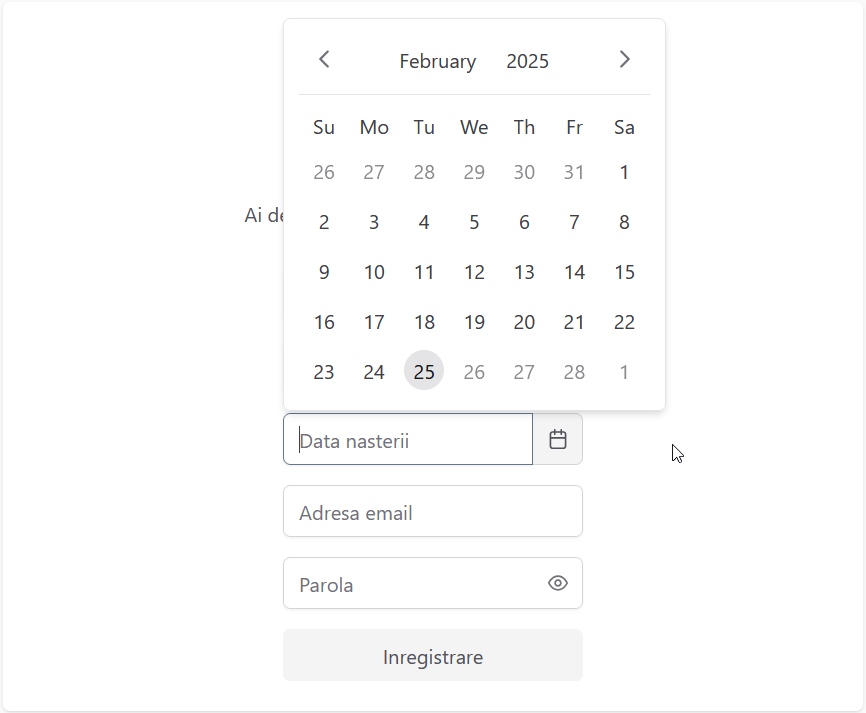
\includegraphics[width=\textwidth,height=0.8\textheight,keepaspectratio]{DatePicker.png}
  \caption{PrimeVue DatePicker component}\label{fig:datepicker}
\end{figure}

\FloatBarrier{}

To ensure control of route access, a simple navigation guard was created using Vue Router. Its role is to protect the routes flagged as requiring authenticatication, performing validation before navigation. An example of this can be seen below:

\begin{lstlisting}[caption=Navigation Guard]
router.beforeEach(async (to) => {
  const authStore = useAuthStore()
  if (to.meta.requiresAuth) {
    await authStore.checkAuth() // Check if user is authenticated
    if (!authStore.isAuthenticated) {
      return { name: 'Login' } // Redirect to login if not authenticated
    }
  } // More code to handle other cases
})
export default router
\end{lstlisting}

Pinia store was used to manage the global authentication state across the application. It enabled access of authentication states across multiple application components, and was used by the Navigation Guard to validate a user's authentication status. The authentication store can be seen below:

\begin{lstlisting}[caption=Pinia Store for Authentication]
export const useAuthStore = defineStore('auth', () => {
  const isAuthenticated = ref(false)
  const user = ref(null)

  async function checkAuth() { // check if user is authenticated
    try {
      const response = await api.get('/me') // return user ID if user is authenticated
      isAuthenticated.value = true // user is authenticated
      user.value = response.data.user
    }
    // More code to handle errors and no authentication
  }
  return { isAuthenticated, user, checkAuth }})
\end{lstlisting}

\subsection{Challenges}

\subsubsection{Lack of experience}

A primary challenge encountered in this sprint was the lack of experience with some of the frameworks and libraries. As such, the development progress moved slower than expected due to the need to consult documentation or researching guides online. In the end, this learning process enabled to establish a solid foundation that would benefit the next sprints' development.

\subsubsection{Implementation decisions}

Another challenge was evaluating implementation options for different elements of the application, such as authentication. Additional time was spent researching the best practices for each feature \- analysing their advantages, disadvantages and ways to implement them in the current system.

\subsection{Requirements completed}

This initial sprint enabled the completion of some of the foundational requirements for this application:

\begin{itemize}
    \item The system must provide a secure login mechanism for patients by using a combination of login and password.
    \item The database must store the user credentials in a secure manner.
    \item The system must be accessible on all modern desktop and mobile-based browsers.
    \item The system must allow patients to add their own personal information, such as name or date of birth.
\end{itemize}

\section{Sprint \#2}

The second sprint focused on implementing system functionality, specifically managing vaccines, allergies and medications. This approach enabled further familiarisation with the frameworks and libraries used in the project, while also establishing design and implementation patterns used in further sprints.

\subsection{Vaccines, allergies and medication management}

Database models were first created for vaccines, allergies and medcations by using SQLModel, followed by corrensponding API endpoints to add, update, delete and view the data. The frontend development used Vue components to create reusable elements, that would be used to display the user added records. These components used other Vue features such as props and emits to pass data and events between elements. An example of the Vaccine Card can be seen below:

\begin{lstlisting}[language=HTML, caption=Vue Vaccine Card Component Example]
<Card class="w-full" :pt="cardStyles">
  <template #title>
    <span class="font-bold text-2xl">{{ name }}</span>
  </template>
  <template #subtitle>
    <div class="flex items-center justify-between">
      <div>
        <span class="font-bold">{{ provider }}</span>
        <span>{{ date_received }}</span> 
      </div>
      <div>
      <Button icon="pi pi-eye" class="p-button-rounded p-button-text"
        @click="emit('showFile', props.id)" v-if="hasCertificate"/>
      <Button icon="pi pi-ellipsis-h" class="p-button-rounded p-button-text"
        @click="toggle"/>
      <Menu ref="menu" :model="items" :popup="true" />
      </div>
    </div>
  </template>
</Card>  
\end{lstlisting}

The VaccineCard component was then easily integrated in its respective page:

\begin{lstlisting}[language=HTML, caption=Using VaccineCard Component]
<VaccineCard
  v-for="vaccine in vaccines"
  :key="vaccine.id" 
  v-bind="vaccine"
  :has-certificate="!!vaccine.certificate"
  @delete="deleteVaccine"
  @open-edit="openEditDialog"
  @show-file="showCertificate"
/>
\end{lstlisting}

\begin{figure}[htbp]
  \centering
  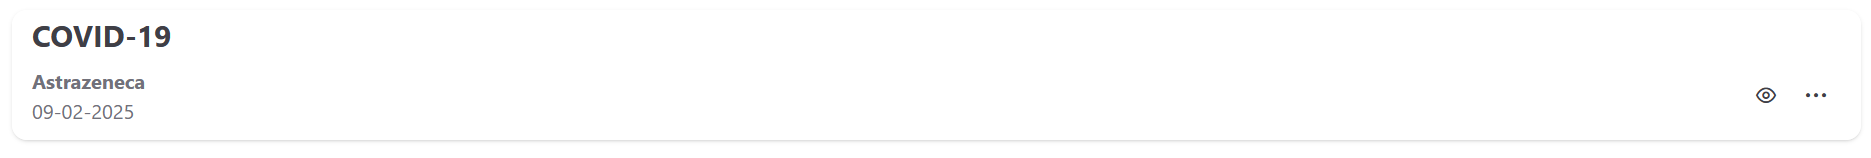
\includegraphics[width=\textwidth,height=0.7\textheight,keepaspectratio]{VaccineCard.png}
  \caption{Vue Vaccine Card component}\label{fig:vaccinecard}
\end{figure}

\FloatBarrier{}

Vue's reactivity system was used to ensure the data was automatically updated whenever any change was made. Examples of the reactivity system in use can be seen below:


\begin{lstlisting}[language=HTML, caption=Vue Reactivity System]
// Will add a vaccine to the vaccines array, which will automatically 
// create a new VaccineCard element
const addVaccine = (vaccine) => {
  vaccines.value.push(vaccine)
}

// Will remove a vaccine from the vaccines array, which will 
// automatically remove the VaccineCard element
const deleteVaccine = (id) => {
  vaccines.value = vaccines.value.filter((vaccine) => vaccine.id !== id)
}
\end{lstlisting}

\subsection{File Uploads feature}

A file upload feature was also implemented in this sprint. It was initially intended for vaccination certificates, but designed to be easily extensible for other future records. This required for a new table to be created in the database, FileUpload, which would contain file metadata. Similarly, a link table for allergies and severities was created to enforce consistency in the names used and allow for easy filtering and sorting on the frontend. The updated ERD diagram, with the new tables, can be seen in figure~\ref{fig:erd_s2}:

\noindent\begin{minipage}{\textwidth}
  \begin{center}
      \rotatebox[origin=c]{270}{
          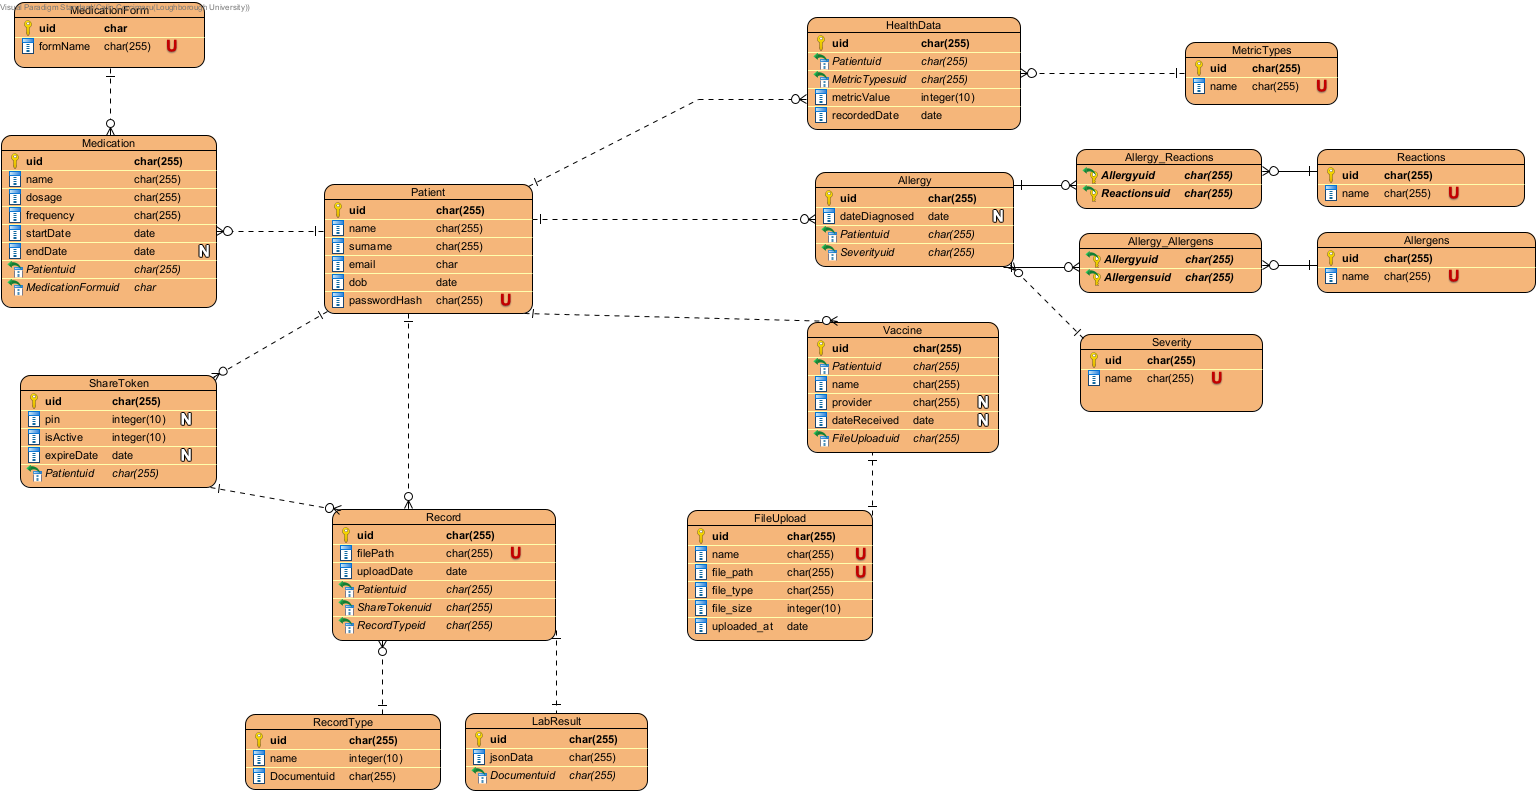
\includegraphics[width=0.95\textheight,keepaspectratio]{ERD_updatedS2.png}
      }
      \captionof{figure}{Updated Entity Relationship Diagram \- Sprint \# 2}\label{fig:erd_s2}
  \end{center}
\end{minipage}

File security was implemented by using AES as the encryption algorithm. It was selected based on a comparative research of existing encryption methods, with AES consistently offering the best balance between security and performance among other symmetric and asymmetric encryption algorithms \parencite{crypt1,crypt2,crypt3}. A symmetric algorithm was used for its implementation simplicity and to prevent users losing access to their files by losing their private key. The key used to encrypt the files was stored in the environment variables. In the interest of time, no rotation system for the key was implemented, however this would be a good feature to add in the future. 

The file upload process can be seen in figure~\ref{fig:fileuploadview} below. It encompasses the following steps:

\begin{enumerate}
  \item File upload to server via multipart form data
  \item Server-side validation of file type and size
  \item File encryption and storage in the file system and database
  \item For retrieval, the file would be streamed via a new endpoint
\end{enumerate}

\begin{figure}[htbp]
  \centering
  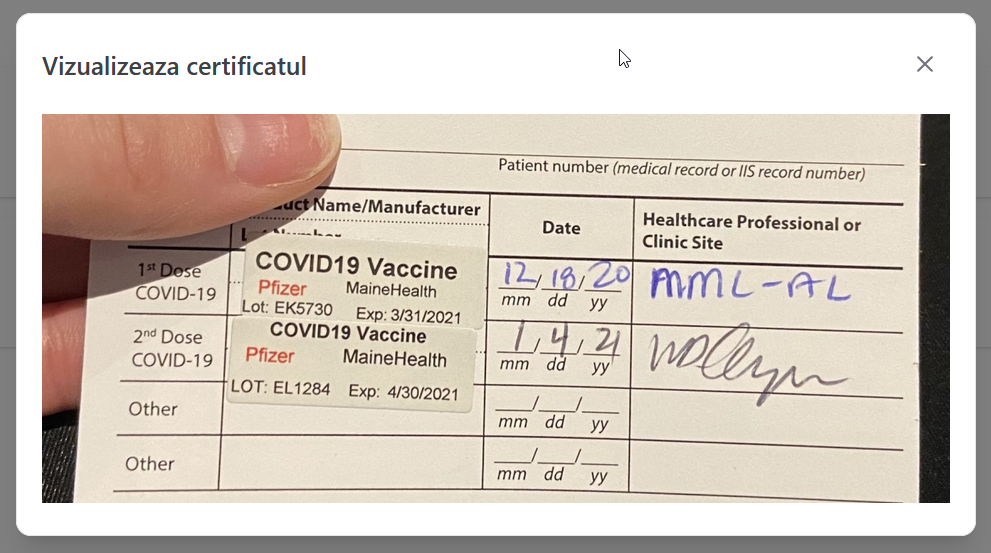
\includegraphics[width=\textwidth,height=0.7\textheight,keepaspectratio]{VaccineCertificate.png}
  \caption{Uploaded Vaccine Certificate}\label{fig:vaccinecertificate}
\end{figure}

\FloatBarrier{}

\begin{figure}[ht]
  \centering
  \subfloat[File Upload Sequence Diagram]{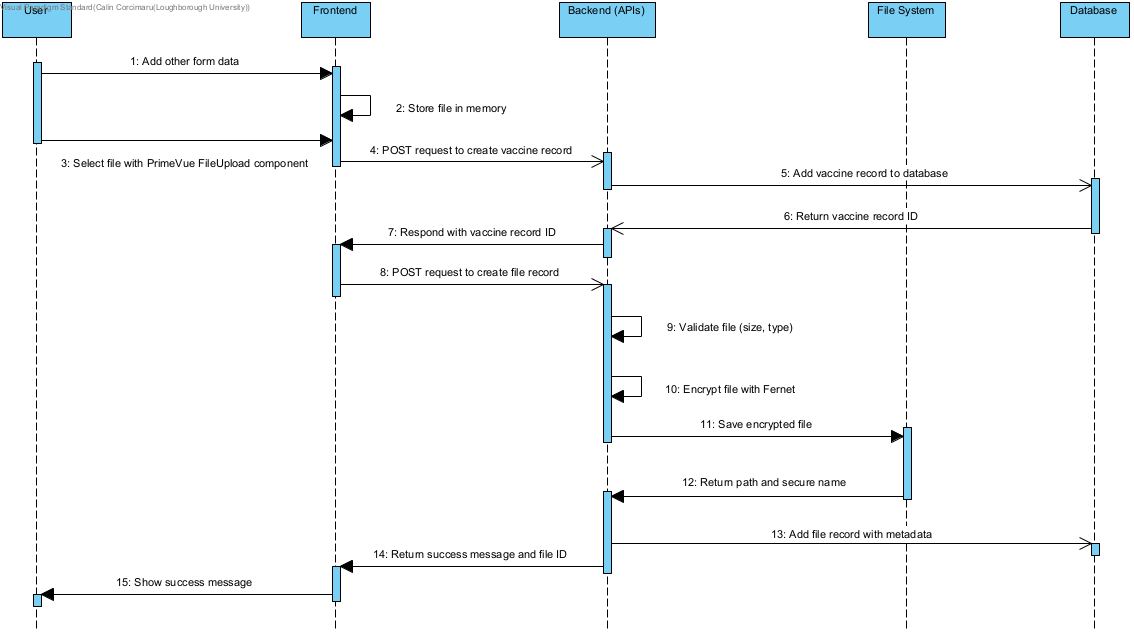
\includegraphics[width=\textwidth]{Sequence_FileUpload.png}\label{fig:seqfileupload}} 
  \\
  \subfloat[File View Sequence Diagram]{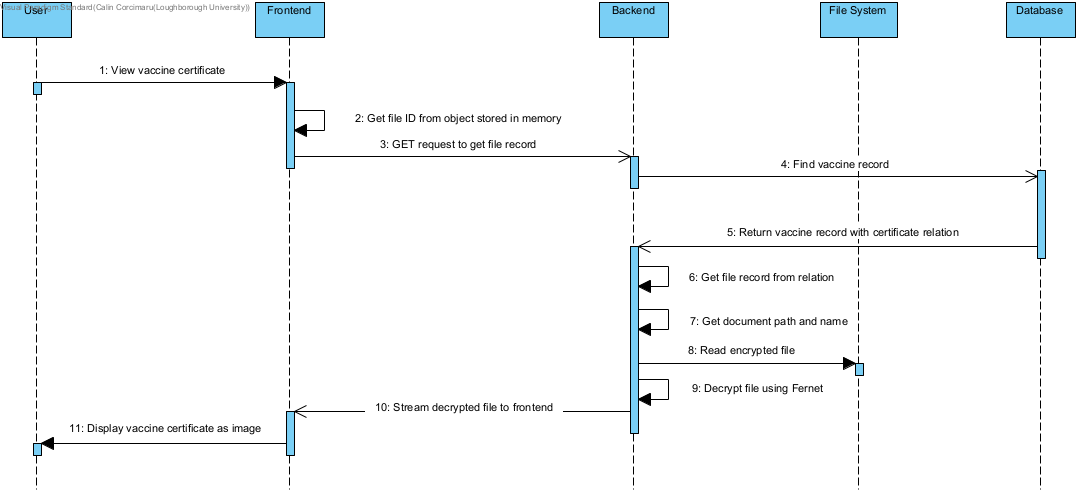
\includegraphics[width=\textwidth]{Sequence_FileView.png}\label{fig:seqfileview}} 
  \caption{Sequence Diagrams for File Upload and File View}\label{fig:fileuploadview}
\end{figure}

\FloatBarrier{}

\begin{lstlisting}[language=Python, caption=File Download Endpoint]
# Get a file by ID
@app.get("/files/{record_type}/{record_id}")
async def get_file(record_type: str, record_id: uuid.UUID, user_id: User = Depends(validate_session), session: Session = Depends(get_session)):    
  # Database query omitted for brevity
  async def get_data_from_file():
    with open(file_record.file_path, "rb") as f:
      encrypted_content = f.read()
    decrypted_content = decrypt_file(encrypted_content)

    yield decrypted_content
    
  return StreamingResponse(
    content=get_data_from_file(),
    media_type=file_record.file_type,
    status_code=status.HTTP_200_OK,
    headers={"Content-Disposition": f"inline; filename={file_record.name}"}
  )
\end{lstlisting}

The frontend was created with both mobile and desktop browsers in mind. This was achieved through using a combination of PrimeVue components TailwindCSS styling. Examples of the allergies page on both desktop and mobile can be seen in figure~\ref{fig:allergiespage}.

\begin{figure}[ht]
  \centering
  \subfloat[Desktop version]{%
      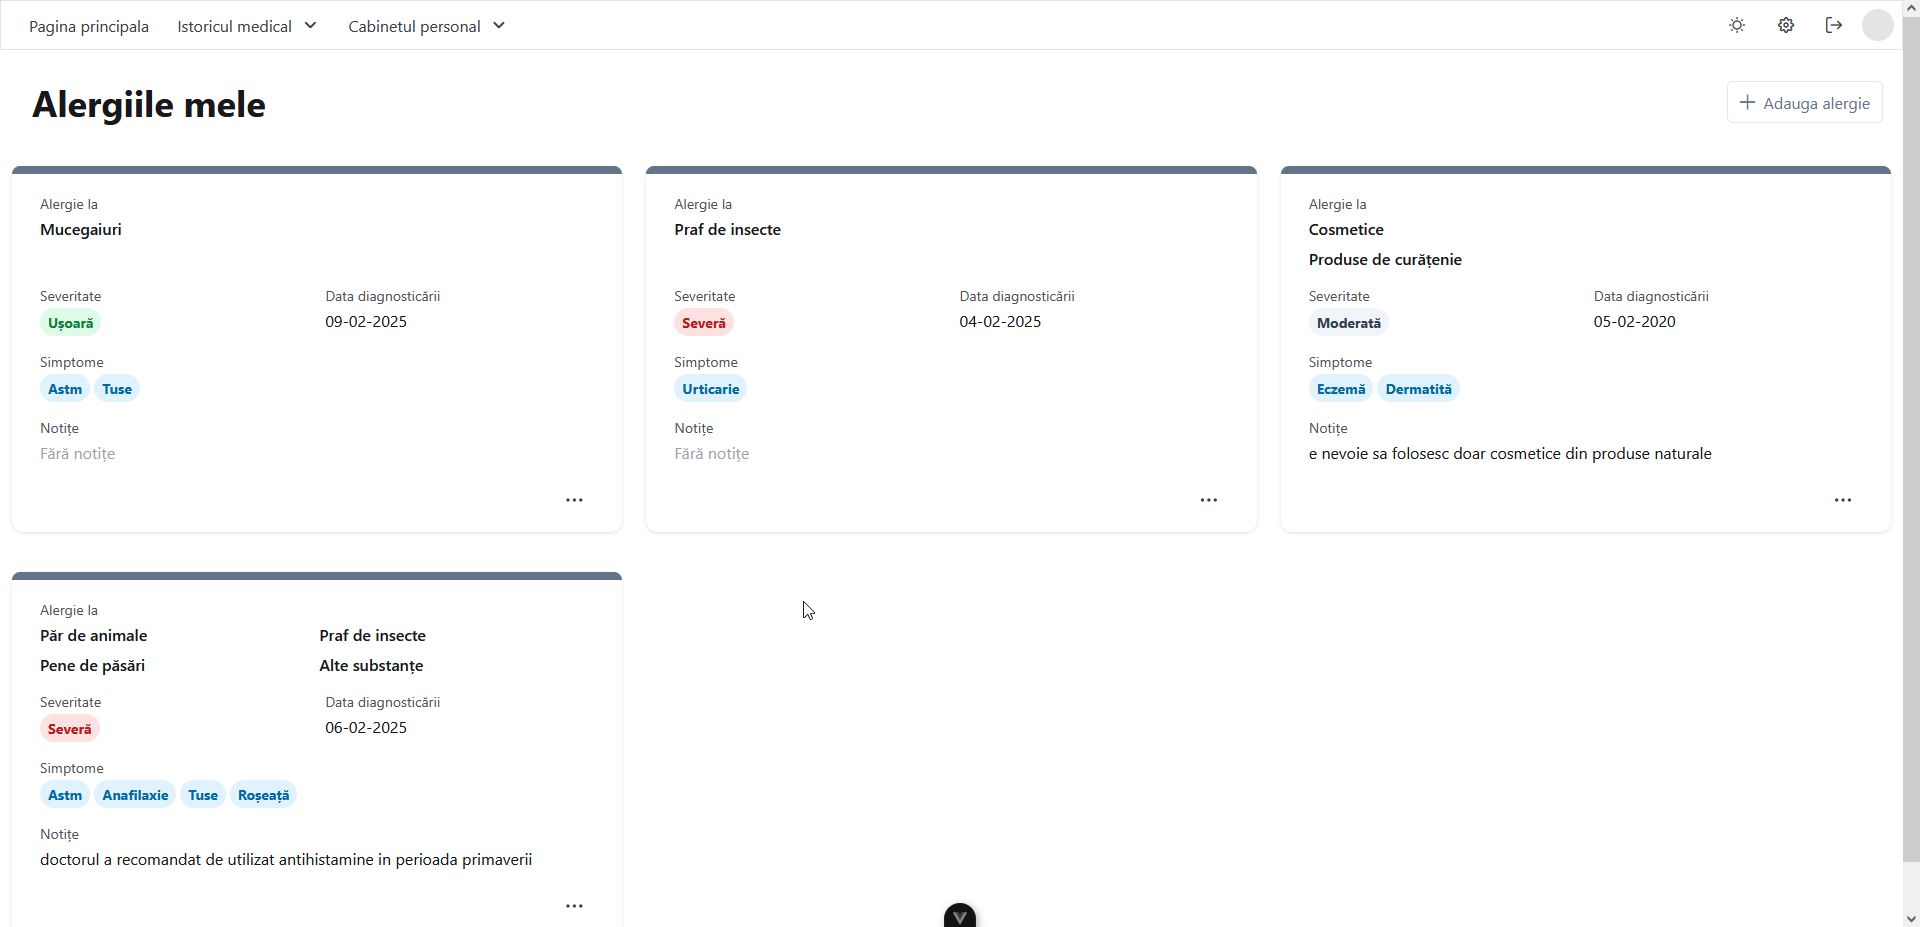
\includegraphics[width=\textwidth]{Desktop_AllergyView.png}%
  }
  \\[\baselineskip]
  \subfloat[Mobile version]{%
      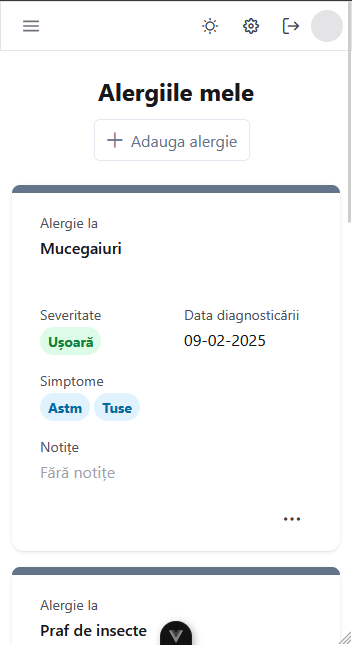
\includegraphics[width=0.4\textwidth]{Mobile_AllergyView.png}%
  }
  \caption{Desktop and Mobile version of the Allergies page}\label{fig:allergiespage}
\end{figure}

\subsection{Challenges}

This sprint encountered its share of challenges. However, tackling them showed that undertaking a more agile approach to the project was beneficial, as the project allowed to embrace change and to be flexible during the development process.

\subsubsection{New functionality integration}

Introducing new functionality in the system, while ensuring compatibility with both the frontend and backend, was the main challenge this sprint. Additional complexity was added by changing existing code or database models to accommodate the new features, which required careful planning and testing to ensure that the new features did not break any existing functionality.

\subsubsection{File Uploads}

Lack of prior experience working with server and client side file handling features was another challenge encountered this sprint. It required additional research, development and testing time to ensure proper implementation and compatibility with the existing system.

\subsubsection{Poor planning \& time management}

The additional complexity brought by the integration of this sprint's feature required more time than initially estimated. As such, poor planning and time management resulted in moving some of the sprint's planned features to the next one, ensuring a rushed development would be avoided.

\subsection{Requirements completed}

The main requirements completed in this sprint were:

\begin{itemize}
    \item The system must store the data in a secure manner, ensuring only the patient and doctor can access the data.
    \item The system must allow patients to upload records in multiple file formats.
    \item The system should allow users to assign uploaded files for all record types.
    \item The system must allow the patient to add their own allergies.
    \item The system must allow the patient to add their own vaccinations.
    \item The system must allow patients to enter their current medication details.
    \item The system must allow patients to add new medication to their list.
\end{itemize}

\section{Sprint \#3}

The third sprint focused on implementing the main dashboard and the vital signs functionality of the system, which would allow patients to add information such as weight or blood pressure in both a tabular and graphical format. Stakeholder feedback from previous sprints also had to be addressed, which included reworking some frontend elements to ensure consistency across application pages.

The features were chosen to be completed this sprint as their implementation would help build proficiency with the frameworks and libraries before tackling more complex functionality in subsequent sprints.

\subsection{User interface rework}

During a presentation of previous sprint results, the stakeholders identified inconsistencies in how information was presented across pages in the application, caused by the different information each record contained. To ensure a consistent view of medical records, PrimeVue's Data View component was implemented. It provided both a grid and list visualisation option, while allowing for customisation of how individual records were displayed. The information displayed was also simplified, to ensure important details were conveyed without distractions. 

An example of the updated allergies page can be seen in figure~\ref{fig:allergiespagev2}. The page now offers both a grid and list view, which can be toggled by the user, creating a more consistent view across different medical records.

\begin{figure}[ht]
  \centering
  \subfloat[Desktop version]{%
      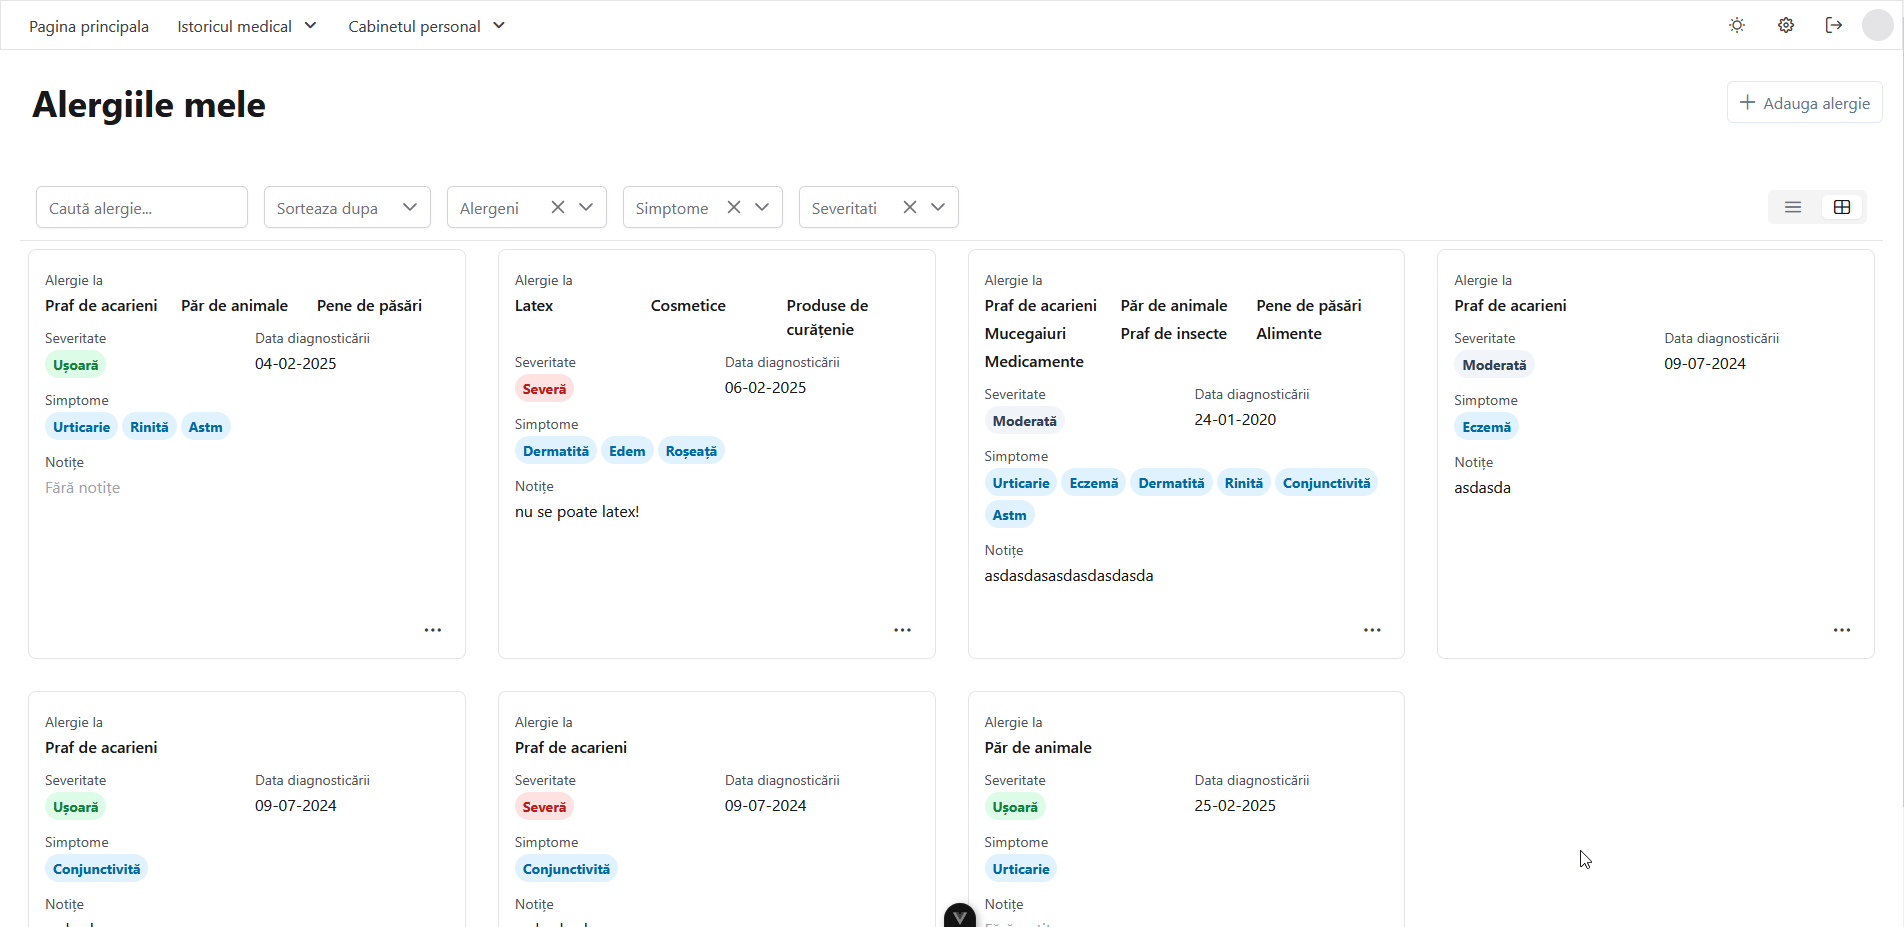
\includegraphics[width=\textwidth]{Desktop_AllergyView_v2.png}%
  }
  \\[\baselineskip]
  \subfloat[Mobile version]{%
      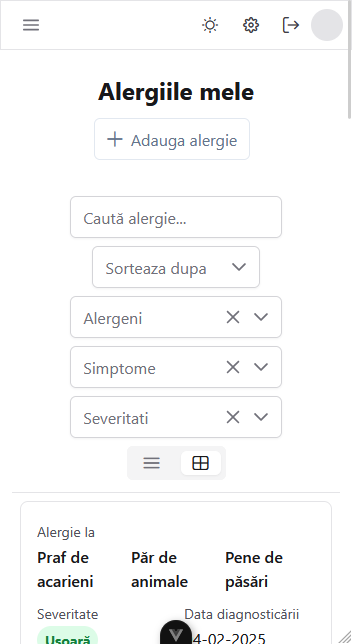
\includegraphics[width=0.4\textwidth]{Mobile_AllergyView_v2.png}%
  }
  \caption{Desktop and Mobile version of the Allergies page \- 2nd version}\label{fig:allergiespagev2}
\end{figure}

\subsection{Filtering and sorting}

Stakeholder feedback also identified the need to filter and sort the information displayed in the application. This was implemented by using Vue's reactivity system, ref and computed functions. It allowed to create complex relationships, which would update variables based on given input or data change. An example of the sorting and filtering functionality can be seen below:

\begin{lstlisting}[language=HTML, caption=Medication Sorting and Filtering]
  const filteredMedicine = computed(() => {
    return props.medications.filter((medication) => {
      return medication.name.toLowerCase().includes(searchQuery.value.toLowerCase())
    })
  })
\end{lstlisting}

\begin{lstlisting}[language=HTML, caption=Allergies Sorting and Filtering]
  const filteredAllergies = computed(() => {
  
  if (selectedAllergens.value.length > 0) {
    return props.allergies.filter((allergy) =>
      allergy.allergens.some((allergen) => selectedAllergens.value.includes(allergen))
    )
  }

  if (selectedReactions.value.length > 0) {
    return props.allergies.filter((allergy) =>
      allergy.reactions.some((reaction) => selectedReactions.value.includes(reaction))
    )
  }

  if (selectedSeverities.value.length > 0) {
    return props.allergies.filter((allergy) =>
      selectedSeverities.value.includes(allergy.severity)
    )
  }  

  return props.allergies.filter((allergy) =>
    allergy.allergens.some((allergen) =>
      allergen.toLowerCase().includes(searchQuery.value.toLowerCase())
    )
  )
})  
\end{lstlisting}

\subsection{Vital signs monitoring}

The vitals signs feature was implemented to add and track basic health metrics such as weight, blood pressure or pulse over time. This addition allowed for the data to be displayed in both a tabular and graphical format to enable track progress over time. To display the data in a tabular and graphical view, the system uses PrimeVue's Data Table component and Chart.js library respectively. To further enhance the feature, current value indicators and trend markers were added to the component to provide a better user experience. Examples of how the Vitals page looks can be seen in figure~\ref{fig:vitalspage} and~\ref{fig:vitalspagegraph}.

\begin{figure}[ht]
  \centering
  \subfloat[Desktop version]{%
      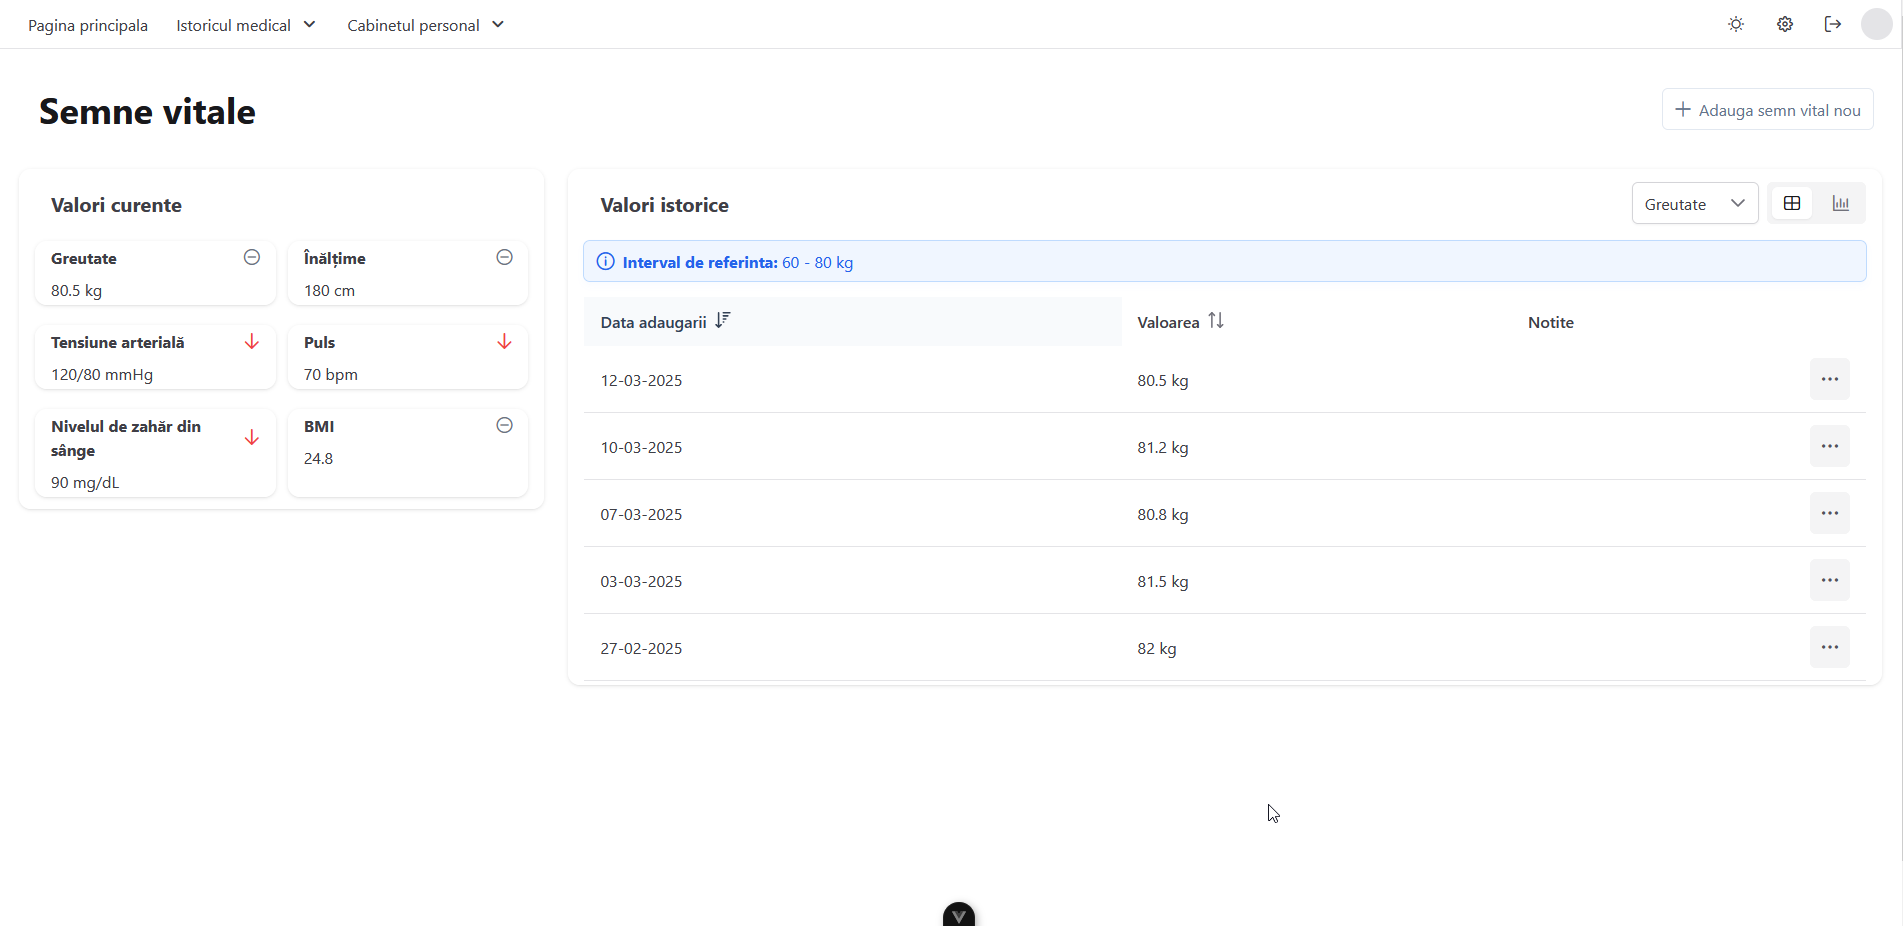
\includegraphics[width=\textwidth]{Desktop_VitalsView.png}%
  }
  \\[\baselineskip]
  \subfloat[Mobile version]{%
      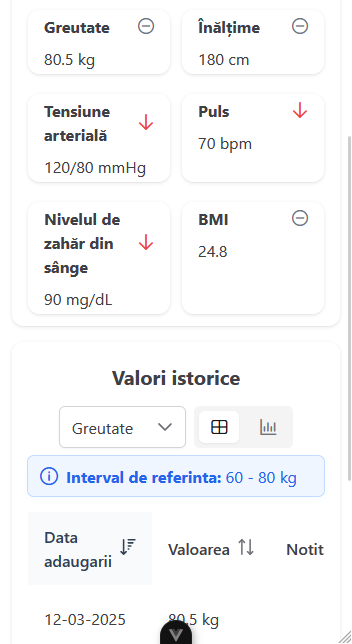
\includegraphics[width=0.4\textwidth]{Mobile_VitalsView.png}%
  }
  \caption{Desktop and Mobile version of the Vitals page}\label{fig:vitalspage}
\end{figure}

\FloatBarrier{}

\begin{figure}[ht]
  \centering
  \subfloat[Desktop version]{%
      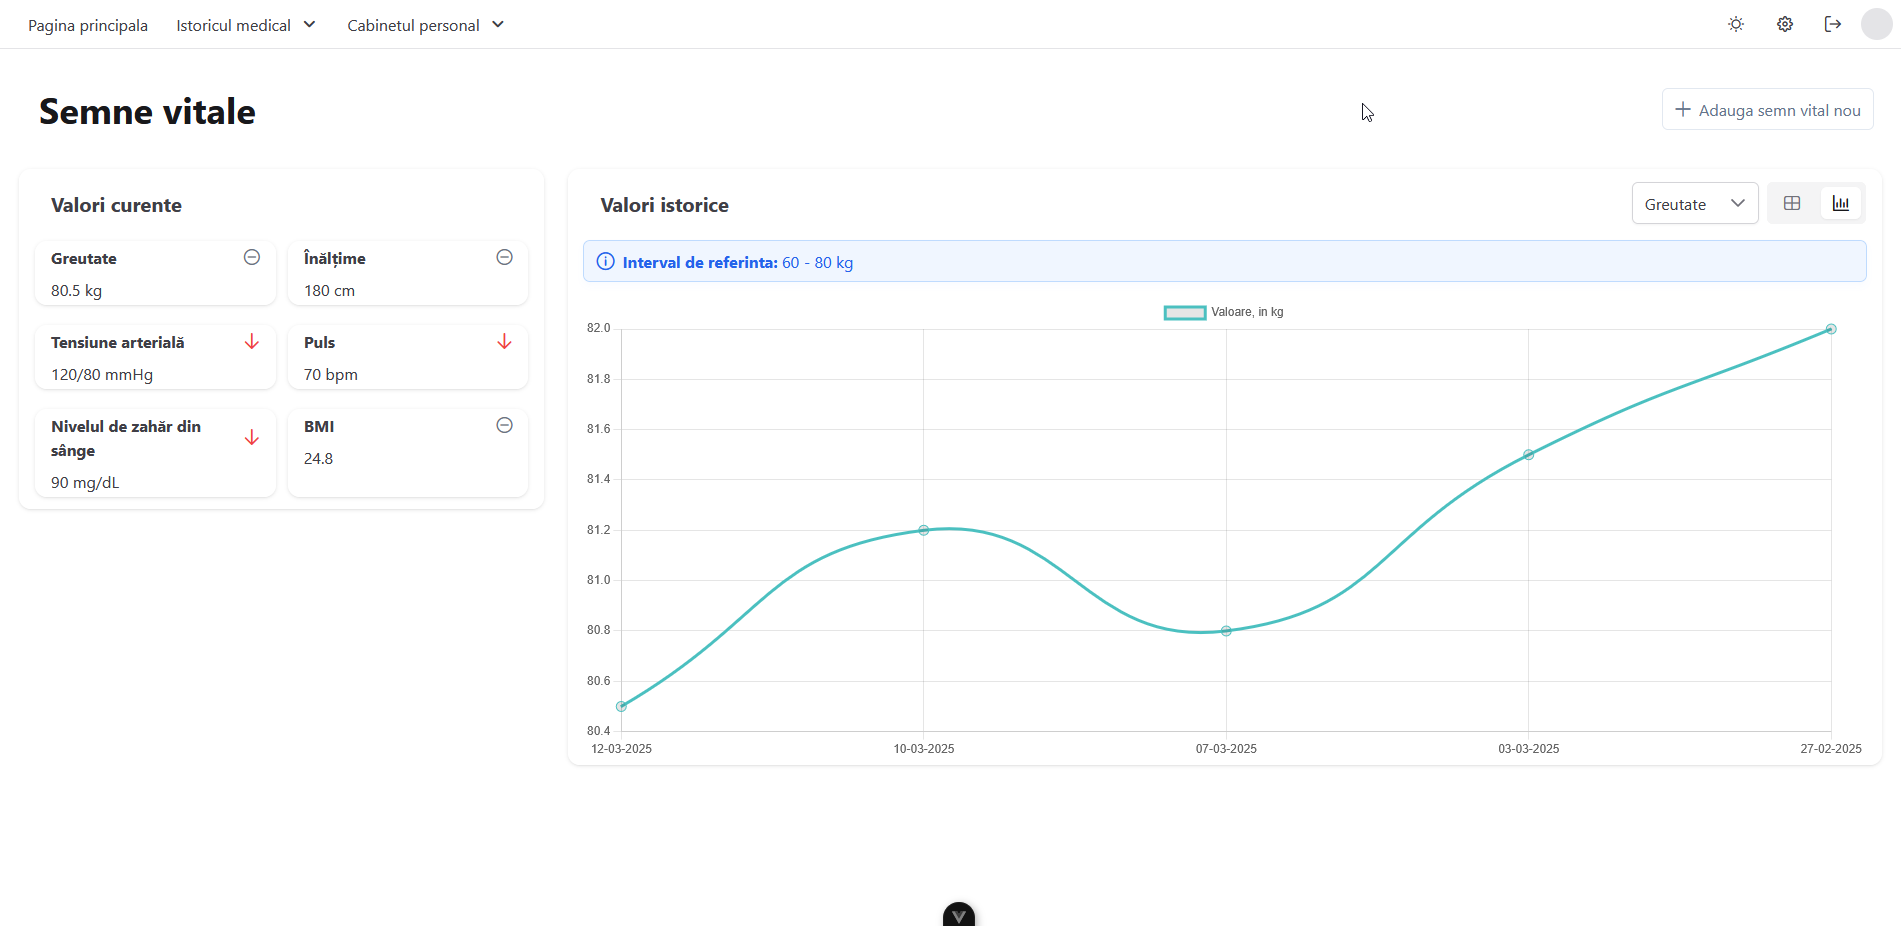
\includegraphics[width=\textwidth]{Desktop_VitalsView_Graph.png}%
  }
  \\[\baselineskip]
  \subfloat[Mobile version]{%
      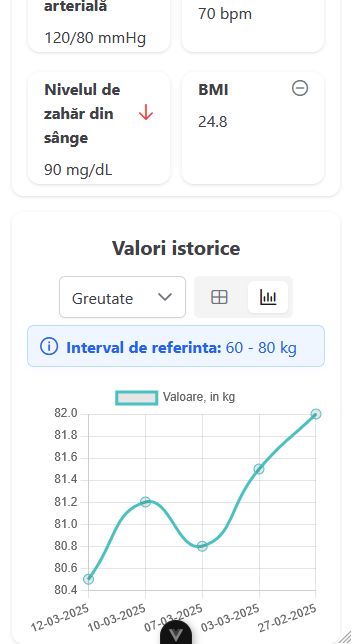
\includegraphics[width=0.4\textwidth]{Mobile_VitalsView_Graph.png}%
  }
  \caption{Desktop and Mobile version of the Vitals page, with Graph}\label{fig:vitalspagegraph}
\end{figure}

\FloatBarrier{}

\subsection{Dashboard implementation}

The dashboard feature was implemented to provide and overview of recent records added to the system. It was designed to present up to 5 recent records for each section, encouraging users to visit the respective page to view more records and details. The display format for each record was kept consistent with their individual pages.

Data Table from PrimeVue was used to create the individual tables for the dashboard sections. Each section was an individual and modular Vue component, which was then imported into the dashboard main file. An example of a section code can be seen below:

\begin{lstlisting}[language=HTML, caption=Vital Signs Dashboard Section Component]
<template>
  <Card :pt="cardStyles" class="h-full">
    <template #title><h2 class="text-xl font-bold p-4">Semne vitale recent adaugate</h2></template>
    <template #content>
      <DataTable :value="props.vitals" removableSort>
        <Column field="name" header="Numele" sortable />
        <Column field="value" header="Valoarea" sortable>
          <template #body="{data}">
            <span v-if="data.value">{{ data.value }} {{ data.unit }}</span>
            <span v-else>{{ data.value_systolic }}/{{ data.value_diastolic }} {{ data.unit }}</span>
          </template>
        </Column>
        <Column field="date_recorded" header="Data adaugarii" sortable>
          <template #body="{data}">{{ data.original_date_recorded }}</template>
        </Column>
      </DataTable>
    </template>
    <template #footer><RouterLink to="/vitale" class="p-button p-button-text">Vezi toate semnele vitale</RouterLink></template>
  </Card>
</template>
\end{lstlisting}

\begin{figure}[ht]
  \centering
  \subfloat[Desktop version]{%
      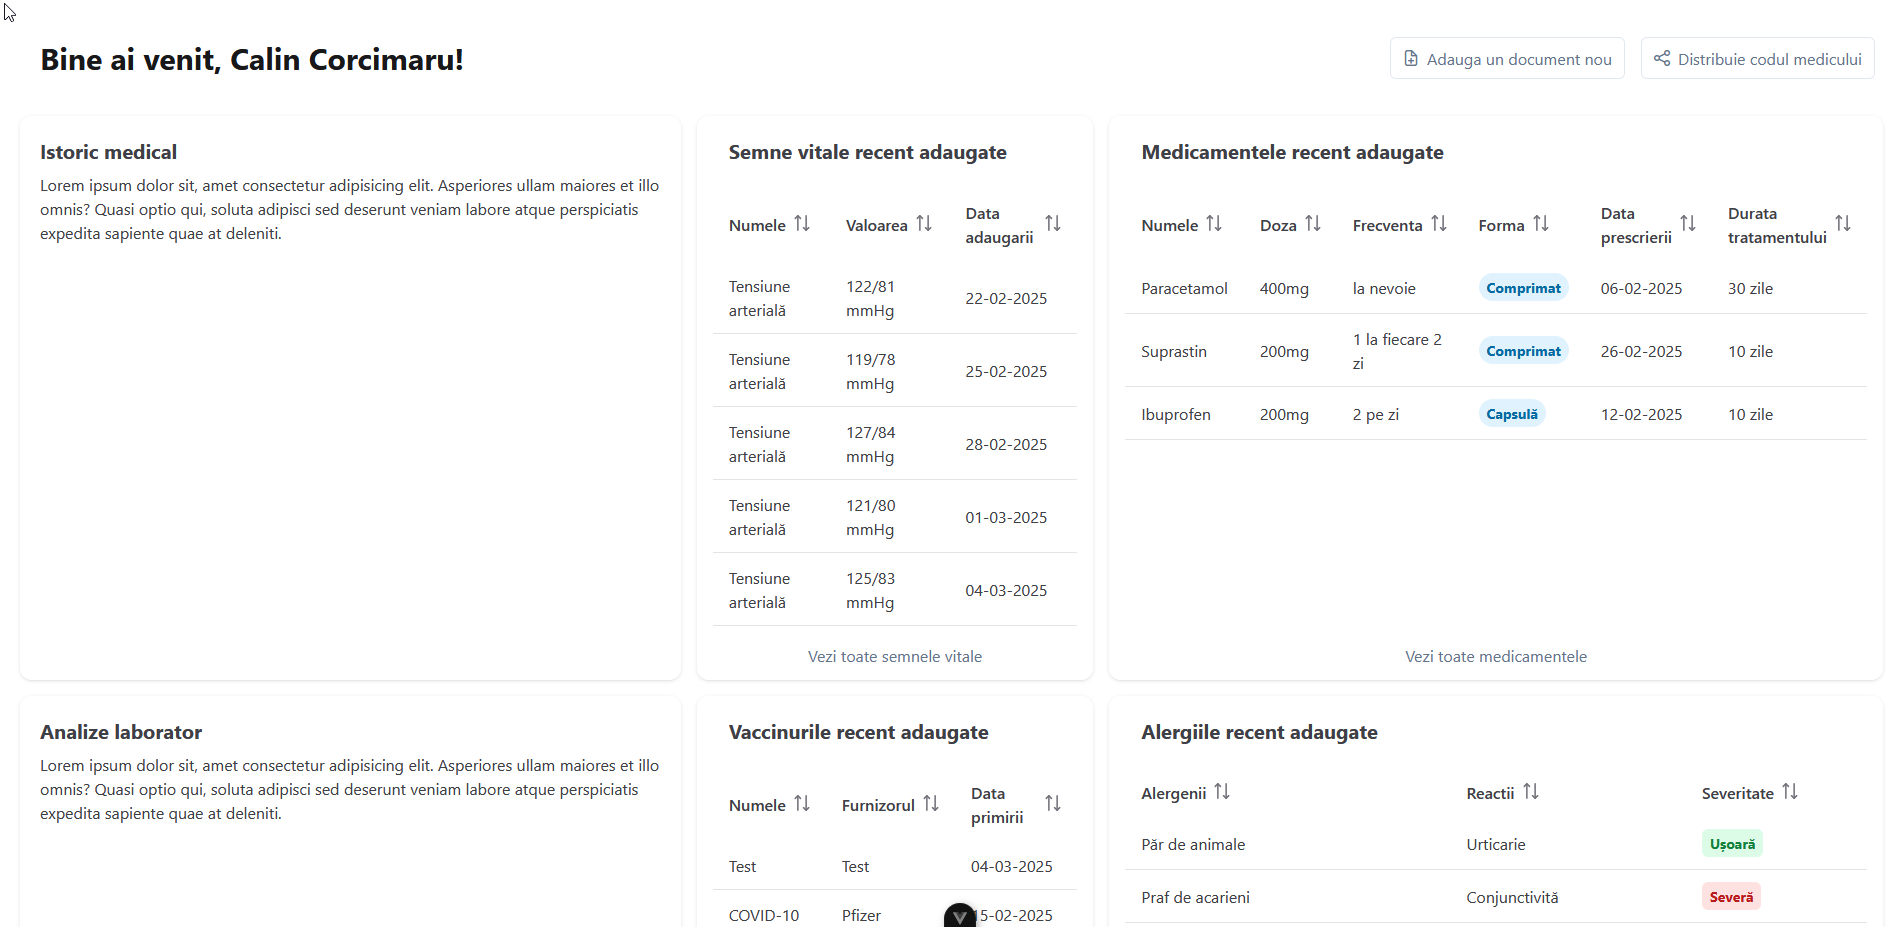
\includegraphics[width=\textwidth]{Desktop_DashboadView.png}%
  }
  \\[\baselineskip]
  \subfloat[Mobile version]{%
      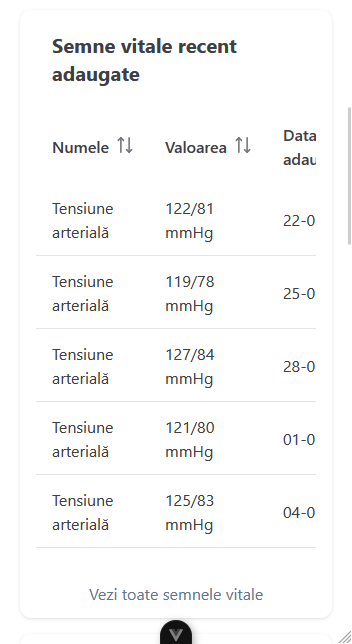
\includegraphics[width=0.4\textwidth]{Mobile_DashboardView.png}%
  }
  \caption{Desktop and Mobile version of the Dashboard page}\label{fig:dashboardpage}
\end{figure}

\FloatBarrier{}

\subsection{Backend changes}

Several database changes were implemented to support the new frontend functionalities. The updated backend diagram can be seen in figure~\ref{fig:erd_s3}. The main changes included:

\begin{itemize}
  \item Addition of a new database table for vital signs, with a separate data type to standardise units and references ranges across values.
  \item Addition of a new date\_added fields to all database tables to differentiate between the clinical date it represents and the date it was added to the system, enabling the ability to sort and query the recently added records.
\end{itemize}

To accommodate the newly added table, changes were made to the vital sign API endpoints. Additional endpoints were also created for the dashboard sections to display their most recent results by using the new date\_added field. The dashboard endpoint can be seen below:

\begin{lstlisting}[language=Python, caption=Dashboard Endpoint]
@app.get("/dashboard", response_model=UserDashboard)
async def get_dashboard(user_id: uuid.UUID = Depends(validate_session), session: Session = Depends(get_session)):
    user = session.get(User, user_id)
    
    if user_id != user.id:
        raise HTTPException(status_code=403, detail="You do not have permission to access this endpoint!")   
    
    newest_vaccines = session.exec(select(Vaccine).where(Vaccine.user_id == user_id).order_by(col(Vaccine.date_added).desc()).limit(5)).all()
    
    # Similar code for allergies, medications and vitals...
    # Response transformation code omitted for brevity

    user_dashboard = UserDashboard(
        id = user.id,
        name = user.name,
        vaccines = vaccines_response,
        allergies = allergies_response,
        vitals = healthdata_response,
        medications = medications_response
    )
    return user_dashboard
\end{lstlisting}

\noindent\begin{minipage}{\textwidth}
  \begin{center}
      \rotatebox[origin=c]{270}{
          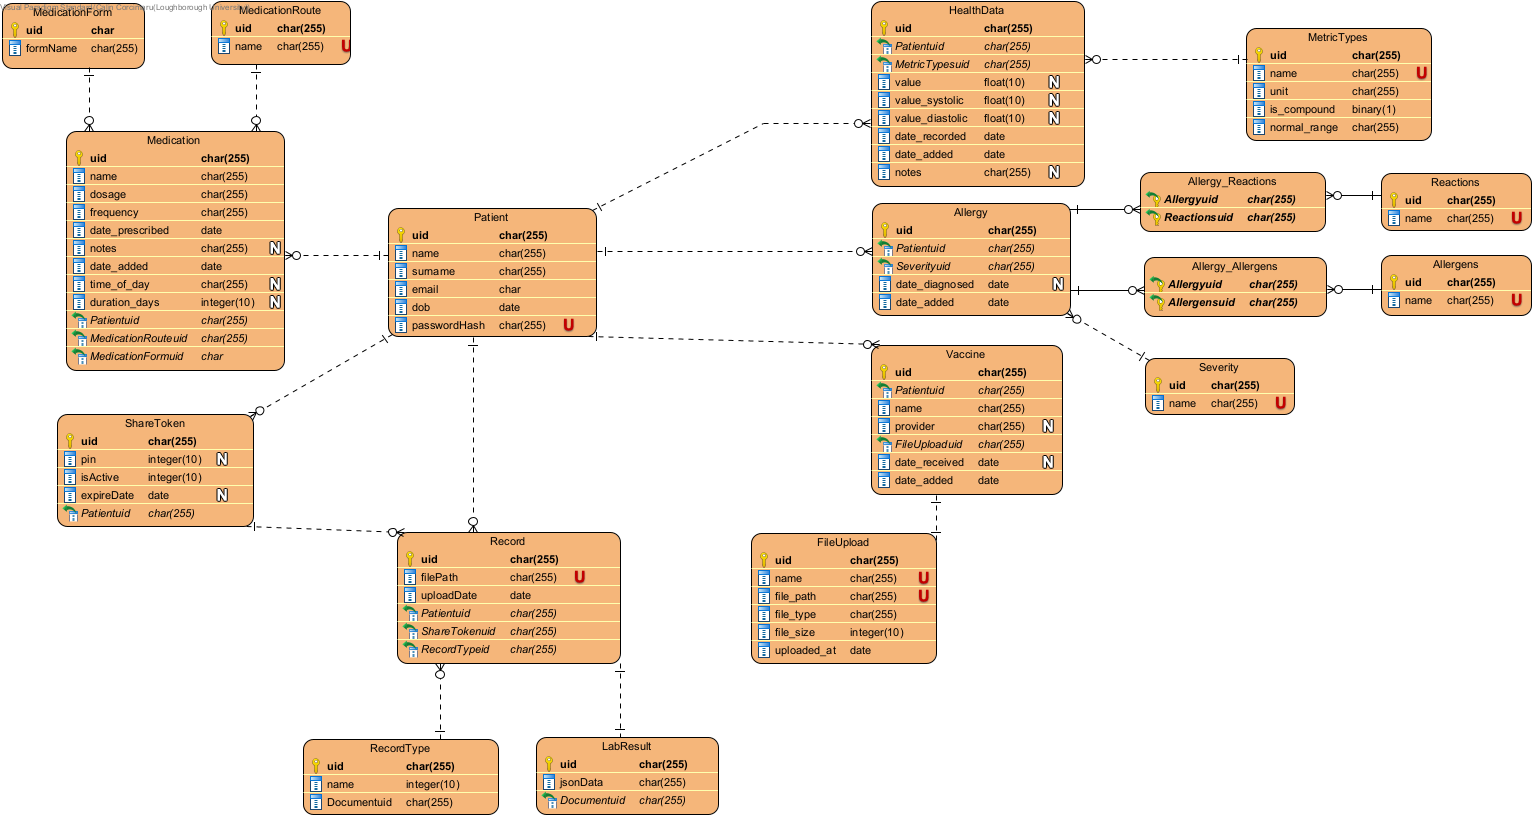
\includegraphics[width=0.95\textheight,keepaspectratio]{ERD_updatedS3.png}
      }
      \captionof{figure}{Updated Entity Relationship Diagram for Sprint \#3}\label{fig:erd_s3}
  \end{center}
\end{minipage}

\subsection{Challenges}

\subsubsection{Scope Creep}

Stakeholder feedback introduced at the start of the sprint led to additional work being done beyond the initial workload planned. Both backend and frontend changes were required to ensure adherence to the new requirements, sapping valuable time and resources from the main sprint objectives. This issue emphasises both the importance of frequent and clear communication with stakeholders, but also the need to establish a clear scope and priority for each sprint.

\subsubsection{Infrequent communication with stakeholders}

Infrequent stakeholder interaction was another issue encountered in this and previous sprints. The unavailability of some stakeholders due to busy schedules as doctors led to some decisions made that later required revision, adding additional workload. As such, more consistent communication with stakeholders was identified as a key improvement necessary for the success of subsequent sprints. 

\subsubsection{Testing limitations}

The lack of experience with automated testing frameworks for the framework resulted in limited testing capability and coverage. Even though testing was still done, albeit manually, not all issues would be immediately caught. This results in intermittent bugs appearing during the development process, which sidetracked the development efforts from the sprint objectives. Additionally, due to time constraints, testing was usually left out at the end or not done at all, leading to even more issues arising unexpectedly in the future.

\subsection{Requirements completed}

\begin{itemize}
    \item The system must have a dashboard view which displays an overview of the most recent information added to the system (latest lab tests, doctor consultations, vaccinations etc).
    \item The system should display the health records in both a list or grid view.
    \item The system should allow the patient to enter vitals information, such as height, weight, blood pressure, etc.
    \item When multiple vital entries are made, the system could display a historical graph of the patient's vitals.
\end{itemize}

\section{Sprint \#4}

The fourth sprint of the project focused on implementing the health records functionality, enabling users to add records such as lab tests, doctor consultations and imaging results. It addresses one of the core requirements of this application, which is to view and manage your medical history in one place. Additional feedback was received from stakeholders at the end of sprint \#3, which included:

\begin{itemize}
    \item Integration of reference ranges for vitals sign graphs
    \item Implementation of date filtering for vital signs data
    \item Adjustment of recent vital signs comparison logic to compare with normal ranges instead
    \item Refinement of dashboard display for allergies and vital signs sections: allergies with moderate and above severities and the most recent value for each vital sign type
\end{itemize}

\subsection{Health Records}

The medical history feature was implemented using PrimeVue's DataTable component to display the data in a tabular format. This allowed for a more structured view of the data, but also enabled the ability to sort and filter by column data thanks to DataTable's built-in functionalities. As such, it was possible to ensure an efficient organisation of data, with consistency across record types. 
An example of the health records page can be seen in figure~\ref{fig:healthrecordspage}.

Advanced filtering options were enabled through DataTable's filtering API, allowing for both global and column-specific filtering options. An example of a filter menu can be seen in figure~\ref{fig:filtermenu}.

Finally, to provide an even better user experience, the document management functionality was enhanced with the ability to display PDF files. This allowed patients to attach files to specific medical records for future reference. On desktop, the files were displayed using the browser's embedded PDF viewer, while on mobile the application would provide a download option to avoid compatibility issues. The code for the PDF viewer can be seen below, with a mobile and desktop example shown in figure~\ref{fig:pdfviewer}.

\clearpage

\begin{lstlisting}[language=HTML, caption=PDF viewer Function for Health]<template>
  <Dialog
    v-model:visible="visible"
    modal
    header="Vizualizeaza fisierul"
    class="w-full md:w-3/4 md:h-3/4"
    @hide="emit('close')">
    <div v-if="metadata?.file_type == 'application/pdf'">
      <object
        :data="`http://localhost:8000/files/medicalhistory/${props.historyId}`"
        type="application/pdf"
        class="w-full h-[70vh] hidden md:block"/>
      <div class="block md:hidden text-center mt-2">
        <a
          :href="`http://localhost:8000/files/medicalhistory/${props.historyId}`"
          target="_blank"
          class="bg-blue-500 text-white px-4 py-2 rounded-md inline-block mb-4">
          Deschide certificatul PDF
        </a>
      </div>
    </div>
    <Image
      v-else
      :src="`http://localhost:8000/files/medicalhistory/${props.historyId}`"
      alt="Fisier consultatie"
      class="w-full h-screen"
      preview/>
  </Dialog>
</template>
\end{lstlisting}

\clearpage

\begin{figure}[ht]
  \centering
  \subfloat[Desktop version]{%
      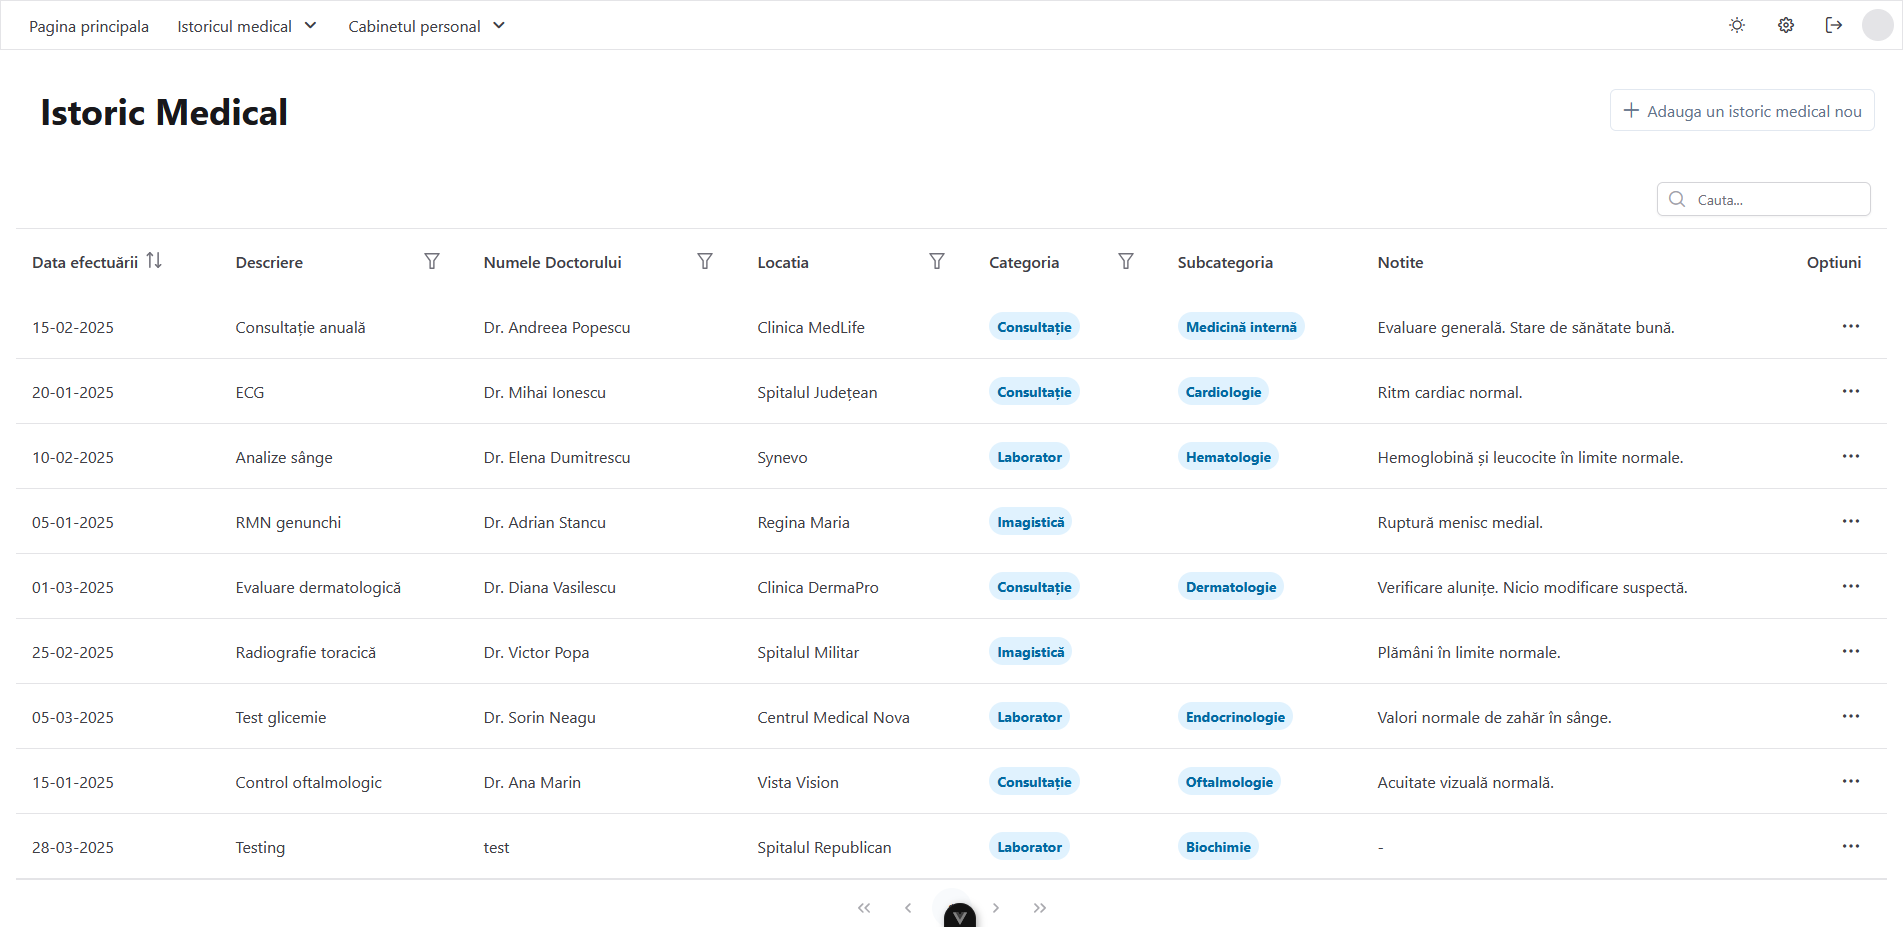
\includegraphics[width=\textwidth]{Desktop_HistoryView.png}%
  }
  \\[\baselineskip]
  \subfloat[Mobile version]{%
      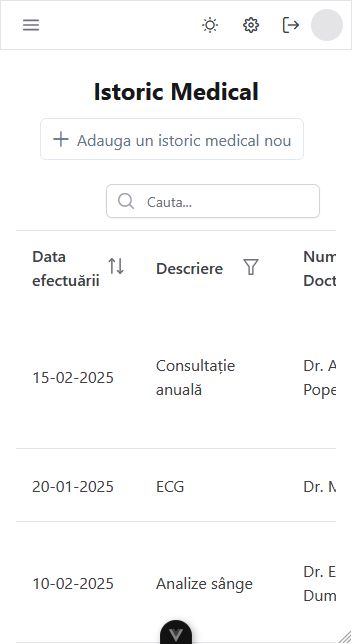
\includegraphics[width=0.4\textwidth]{Mobile_HistoryView.png}%
  }
  \caption{Desktop and Mobile version of the History page}\label{fig:healthrecordspage}
\end{figure}

\begin{figure}[ht]
  \centering
  \subfloat[Desktop version]{%
      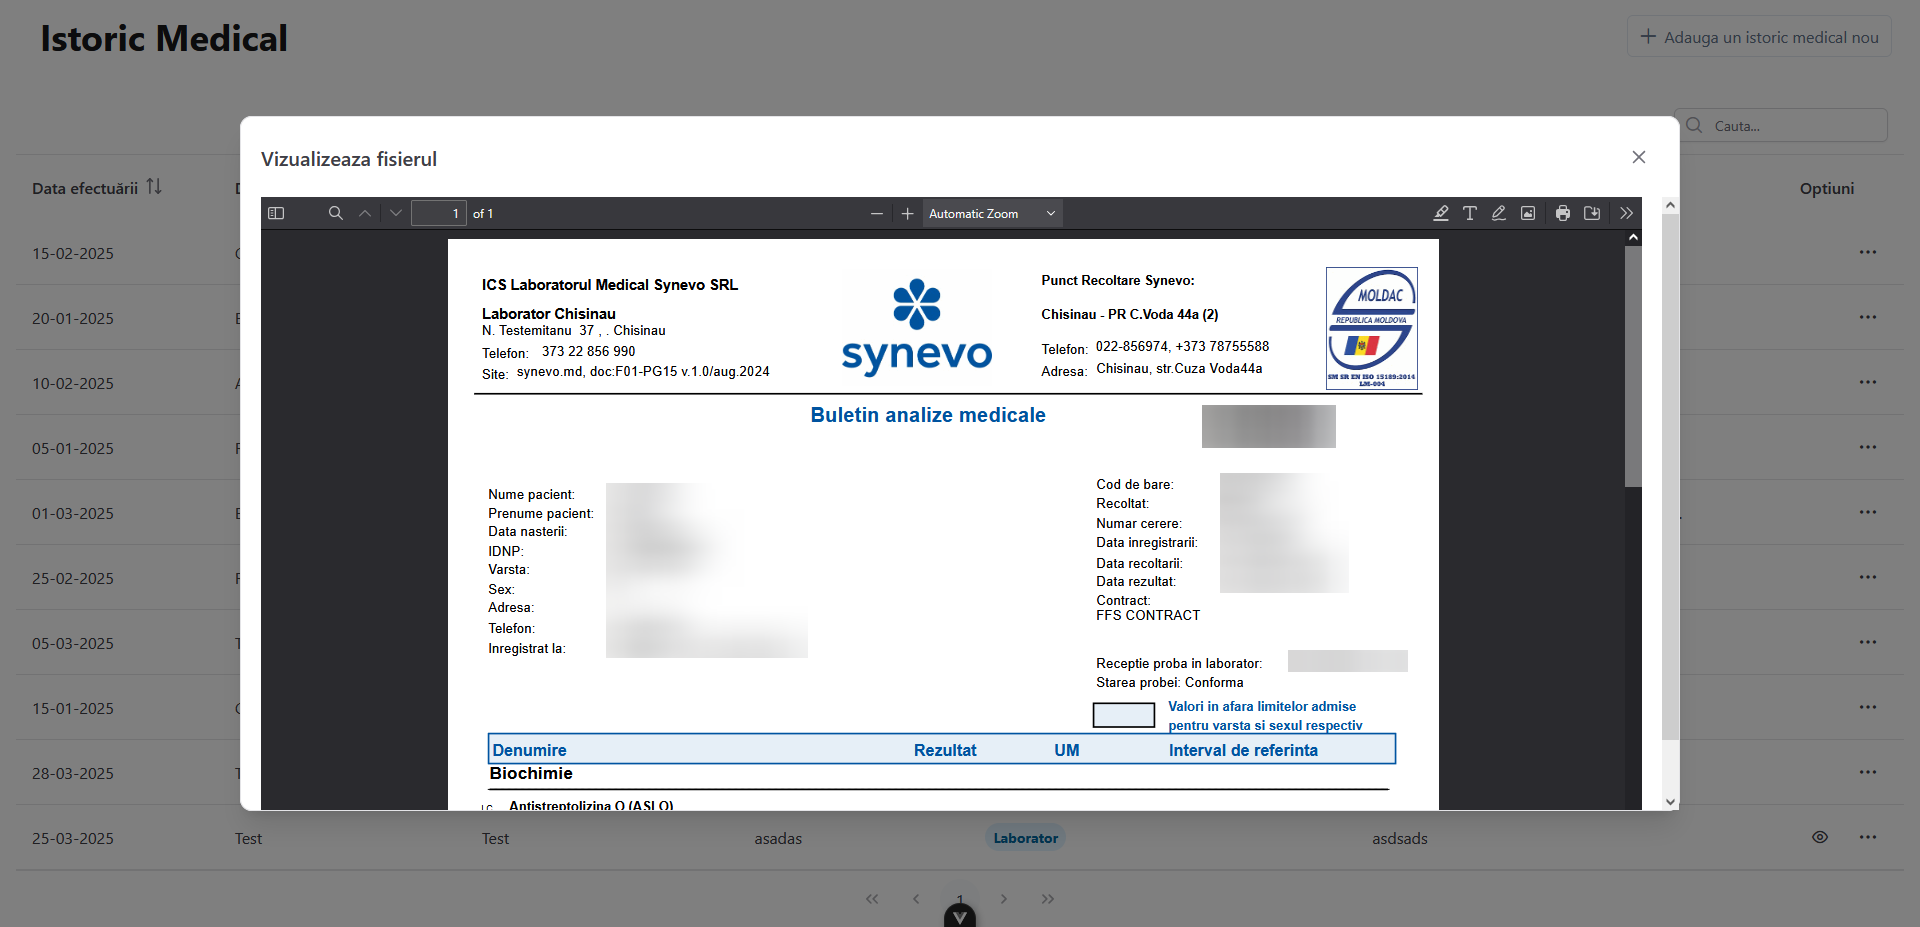
\includegraphics[width=\textwidth]{Desktop_History_PDF.png}%
  }
  \\[\baselineskip]
  \subfloat[Mobile version]{%
      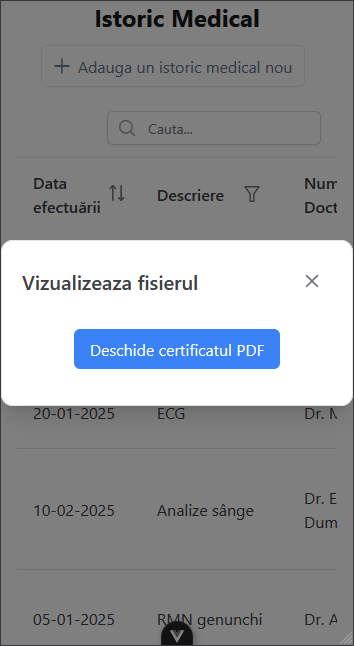
\includegraphics[width=0.4\textwidth]{Mobile_History_PDF.png}%
  }
  \caption{Desktop and Mobile version of the PDF viewer}\label{fig:pdfviewer}
\end{figure}

\FloatBarrier{}

\begin{figure}[htbp]
  \centering
  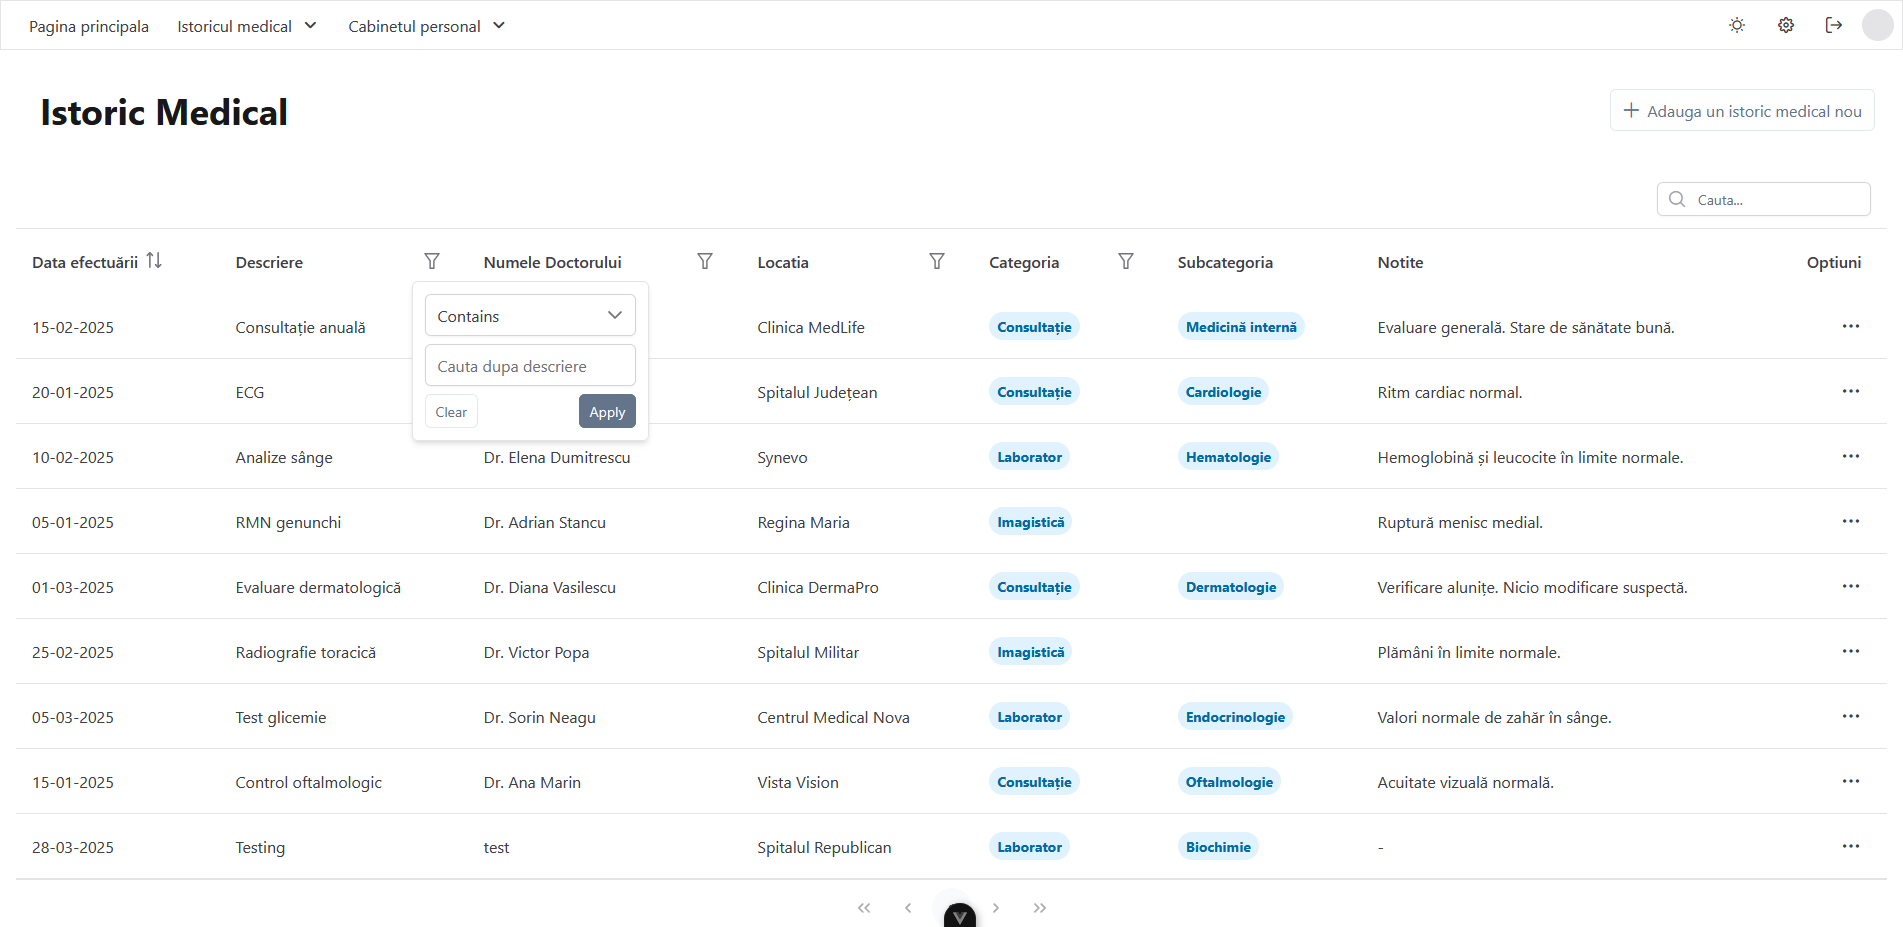
\includegraphics[width=\textwidth]{Desktop_HistoryView_Filter.png}
  \caption{Filter Menu for Health Records}\label{fig:filtermenu}
\end{figure}

\subsection{Backend changes}

To accommodate the medical history feature, the database was extended with new tables to support record organisation, which include a core table for record metadata, a table for primary classification (into consultation, laboratory or imagining) and secondary tables for consultation specialties and test types. The new ERD diagram can be seen in figure~\ref{fig:erd_s4}.

Additionally, API endpoints were created to allow the user to add, edit and delete health records. To promote reusability within the system, the file management endpoints created in sprint \#2 were reused for the medical history feature. 

\noindent\begin{minipage}{\textwidth}
  \begin{center}
      \rotatebox[origin=c]{270}{
          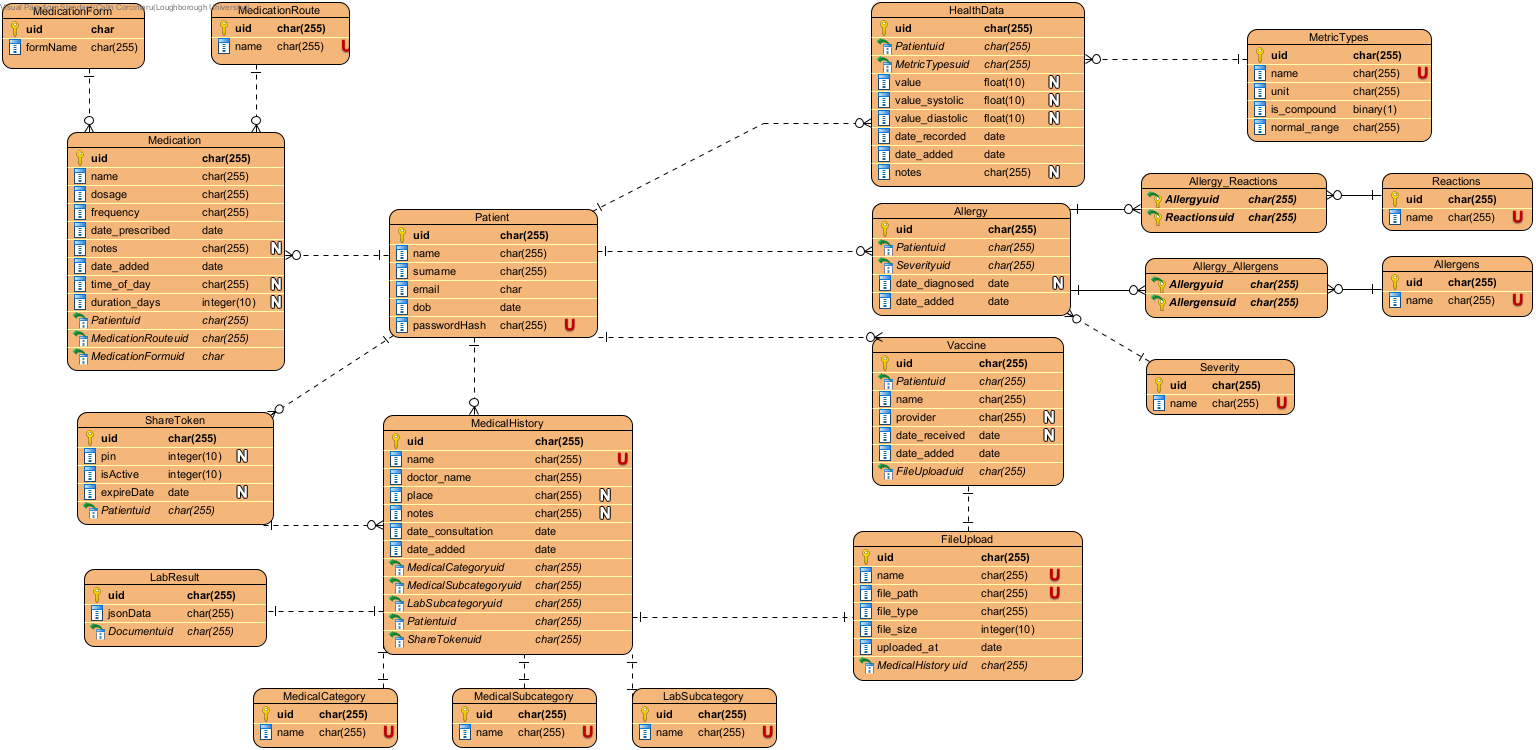
\includegraphics[width=0.95\textheight,keepaspectratio]{ERD_updatedS4.png}
      }
      \captionof{figure}{Updated Entity Relationship Diagram \- Sprint \#4}\label{fig:erd_s4}
  \end{center}
\end{minipage}

\subsection{Work on stakeholder feedback}

Several changes to the user interface were implemented based on stakeholder feedback. The biggest change was the addition of `normal range' boundaries to the graph views for some vital sign types, providing immediate context and feedback for vital sign results. Additionally, a date filter was introduced on the page, allowing users to filter the data based on selected date ranges. Finally, the computation logic for recent vital sign trends was changed to utilise their respective normal ranges to dictate their trend, instead of the previous value. Overall, these changes were made to improve the user experience and provide more context for the data displayed. Their implementation can be seen below in figure~\ref{fig:vitalchanges}.

\begin{figure}[htbp]
  \centering
  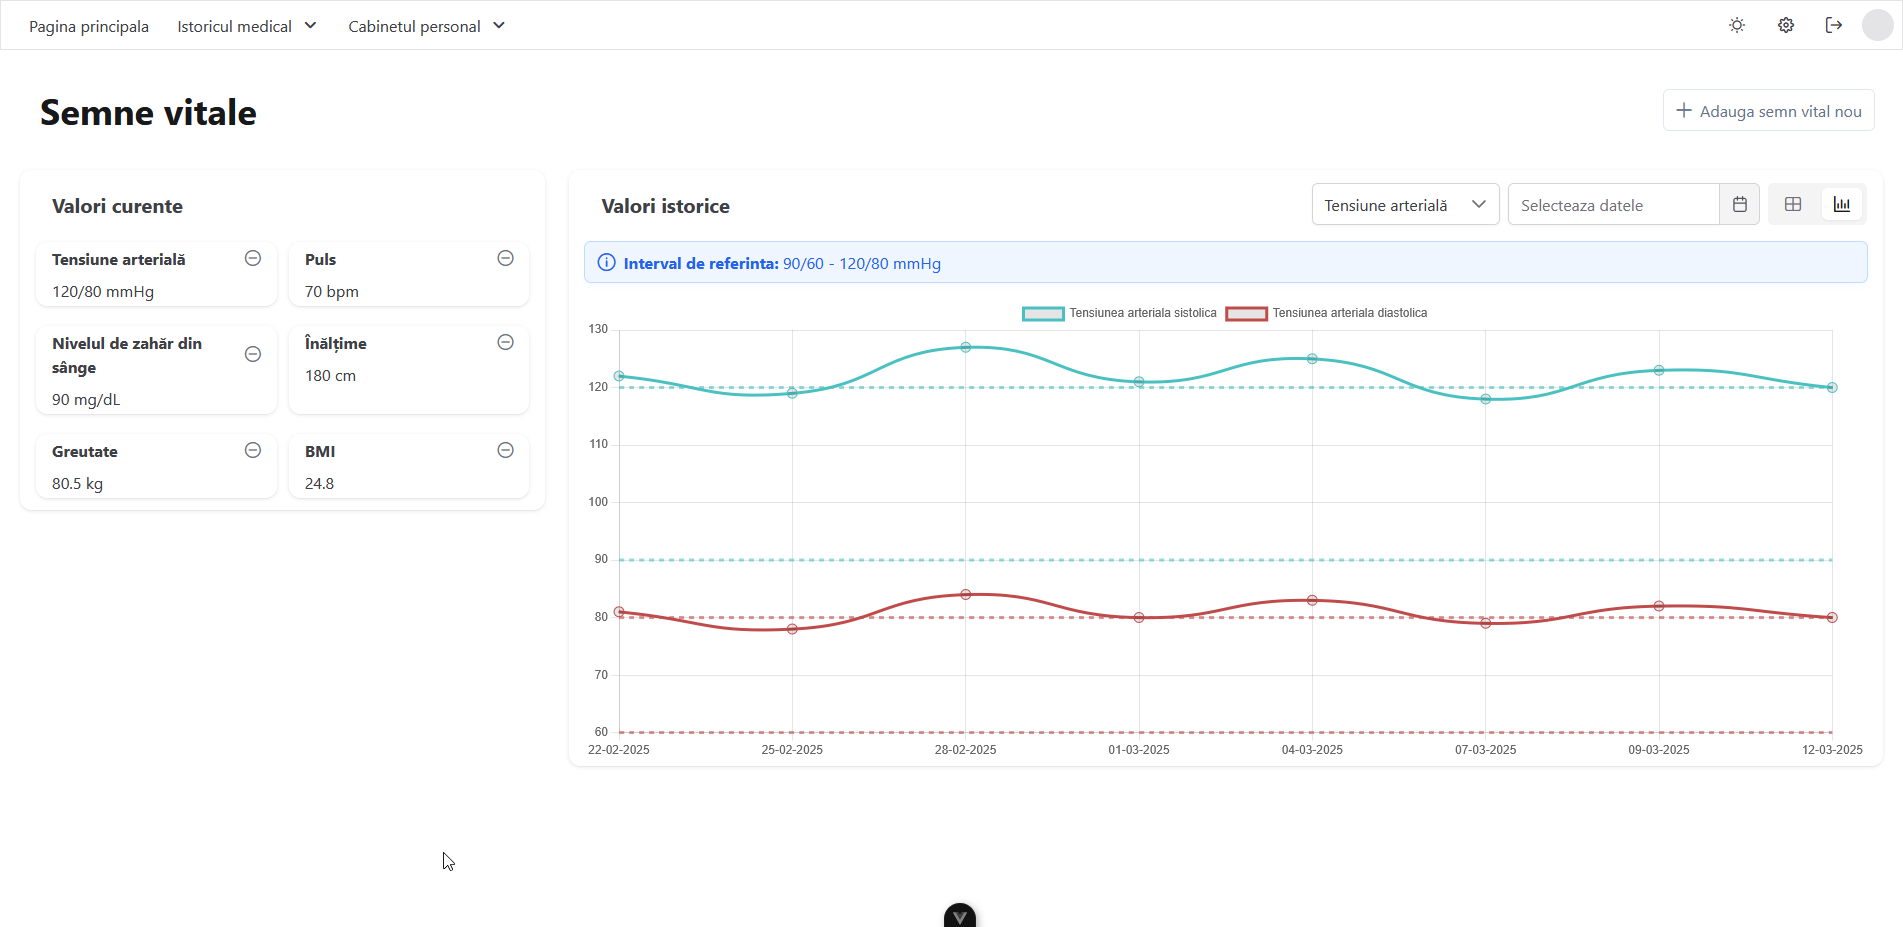
\includegraphics[width=\textwidth]{Desktop_Vitals_Updated.png}
  \caption{Updated Vitals View based on stakeholder feedback}\label{fig:vitalchanges}
\end{figure}

\FloatBarrier{}

The main dashboard view was also optimised to display more accurate and relevant information in some of the existing sections. For vitals signs, only the most recent value for each type was now shown in the dashboard, alongside their trend indicator. For the allergies section, it was changed to only display records with a severity of `moderate' and above to prioritise showing more severe (and more clinically important) cases of a patient's allergies. The new dashboard can be seen in figure~\ref{fig:dashboardchanges}.

\begin{figure}[htbp]
  \centering
  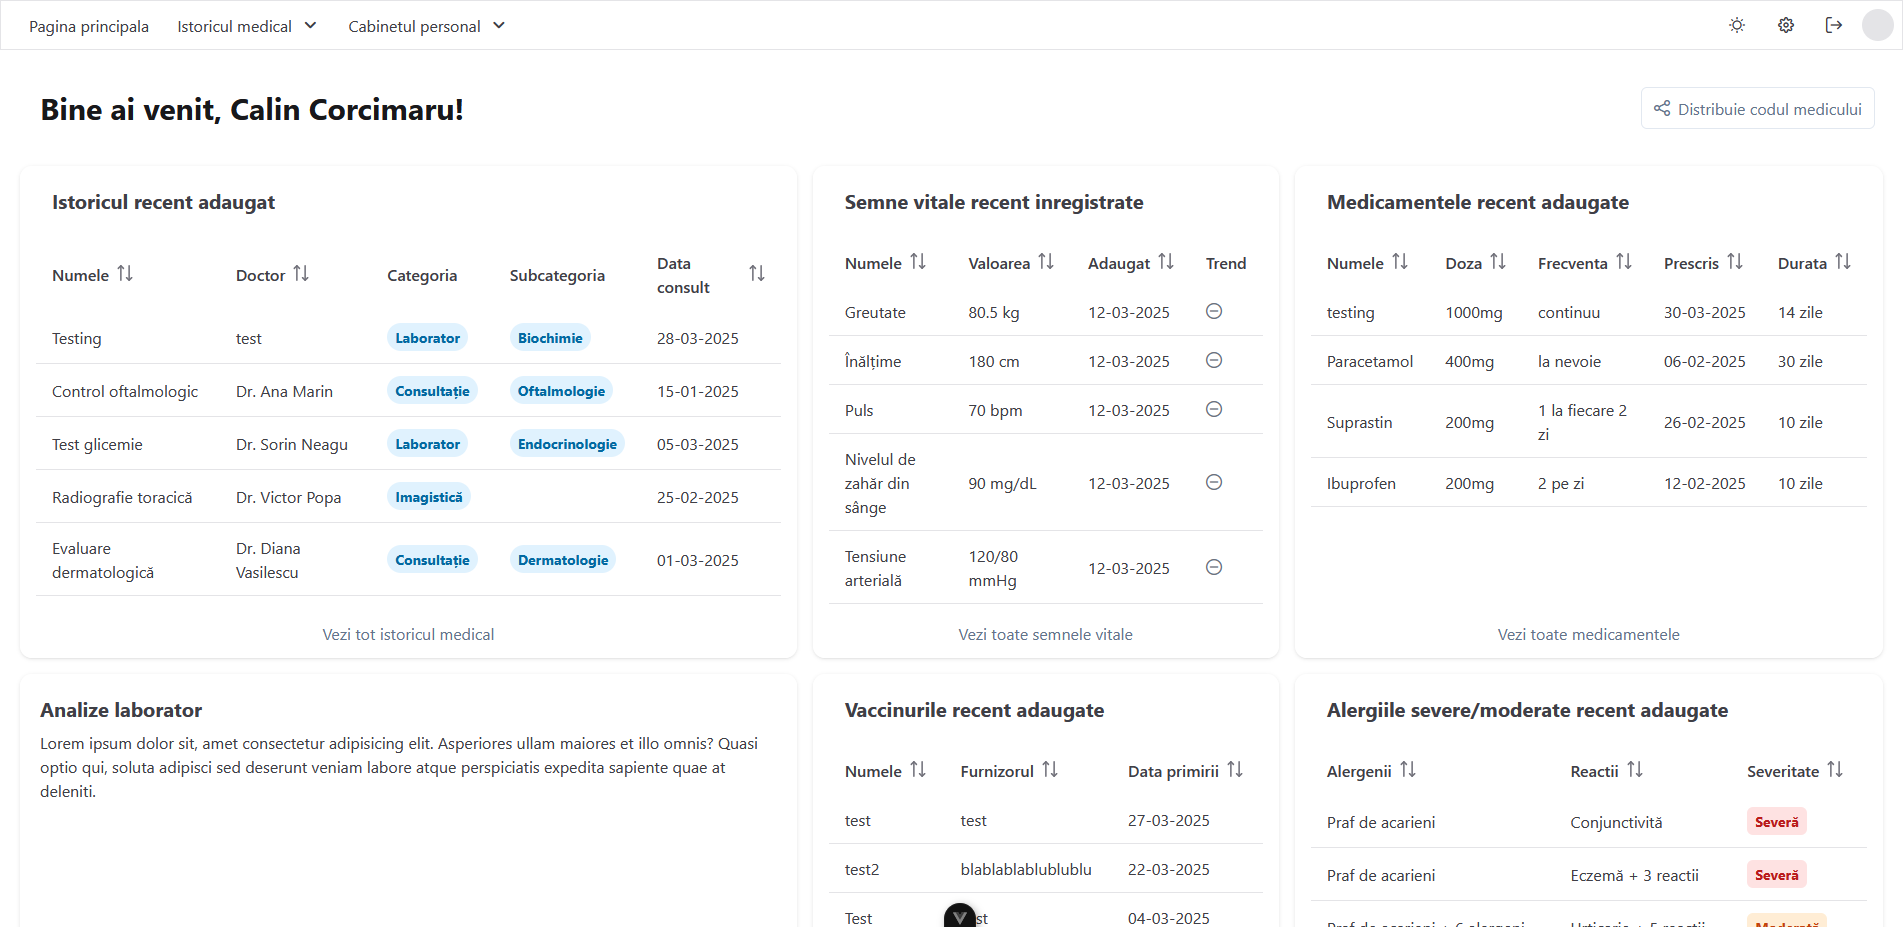
\includegraphics[width=\textwidth]{Desktop_DashboardView_Updated.png}
  \caption{Updated Dashboard View based on stakeholder feedback}\label{fig:dashboardchanges}
\end{figure}

\FloatBarrier{}

\subsection{Challenges}

The primary challenge encountered during this sprint was, interestingly enough, unrelated to any technical implementation issues. Instead, an unexpected period of illness resulted in approximately one week lost of development time, leading to a reduced feature output for this sprint. As such, some of the unfinished worked had to be transferred to the next sprint's backlog.

\subsection{Requirements completed}

\begin{itemize}
  \item The system must allow the patient to specify and categorise the type of document they are uploading (lab test, doctor consultation, etc).
  \item The system must allow patients to upload their own medical records in a variety of formats (PDF, DOC, etc).
  \item The system must display the patient's history in a chronological order in the form of a timeline.
  \item When viewing doctor consultations, the system should divide them into categories based on the domain of the doctor (cardiology, neurology, etc).
  \item The system must allow the patient to add a description of the document they are uploading.
  \item The system should allow the patient to add a date for the document they are uploading.
  \item The system should allow the patient to add a location for the document they are uploading.
  \item The system should allow the patient to add the doctor name for the document they are uploading.
  \item The system should allow the patient to sort and filter the documents based on the type of document, date, location, and doctor name. 
\end{itemize}

\section{Sprint \#5}

The fifth sprint focused on implementing an automated lab test data extraction system that utilised a MLLM to process uploaded lab result documents. This feature represented an incredible innovation within this application, as it enabled automatic extraction of test results from documents, with minimal manual intervention. Being a continuation of the work done in the previous sprint, some of the initial work required for the implementation of this feature was already completed. This allowed for easier and faster development of the lab extraction functionality, which was completed as per the initially agreed requirements and wireframes, with minor changes to how the lab results were displayed on the frontend. 

The sequence diagram for the lab tests extraction process can be seen in figure~\ref{fig:sequence_lab}. It displays how a user would interact with the system when uploading a lab result document, how the system processes the filem sends it to the MLLM API, and how the response is then received and displayed to the user.

\begin{figure}[htbp]
  \centering
  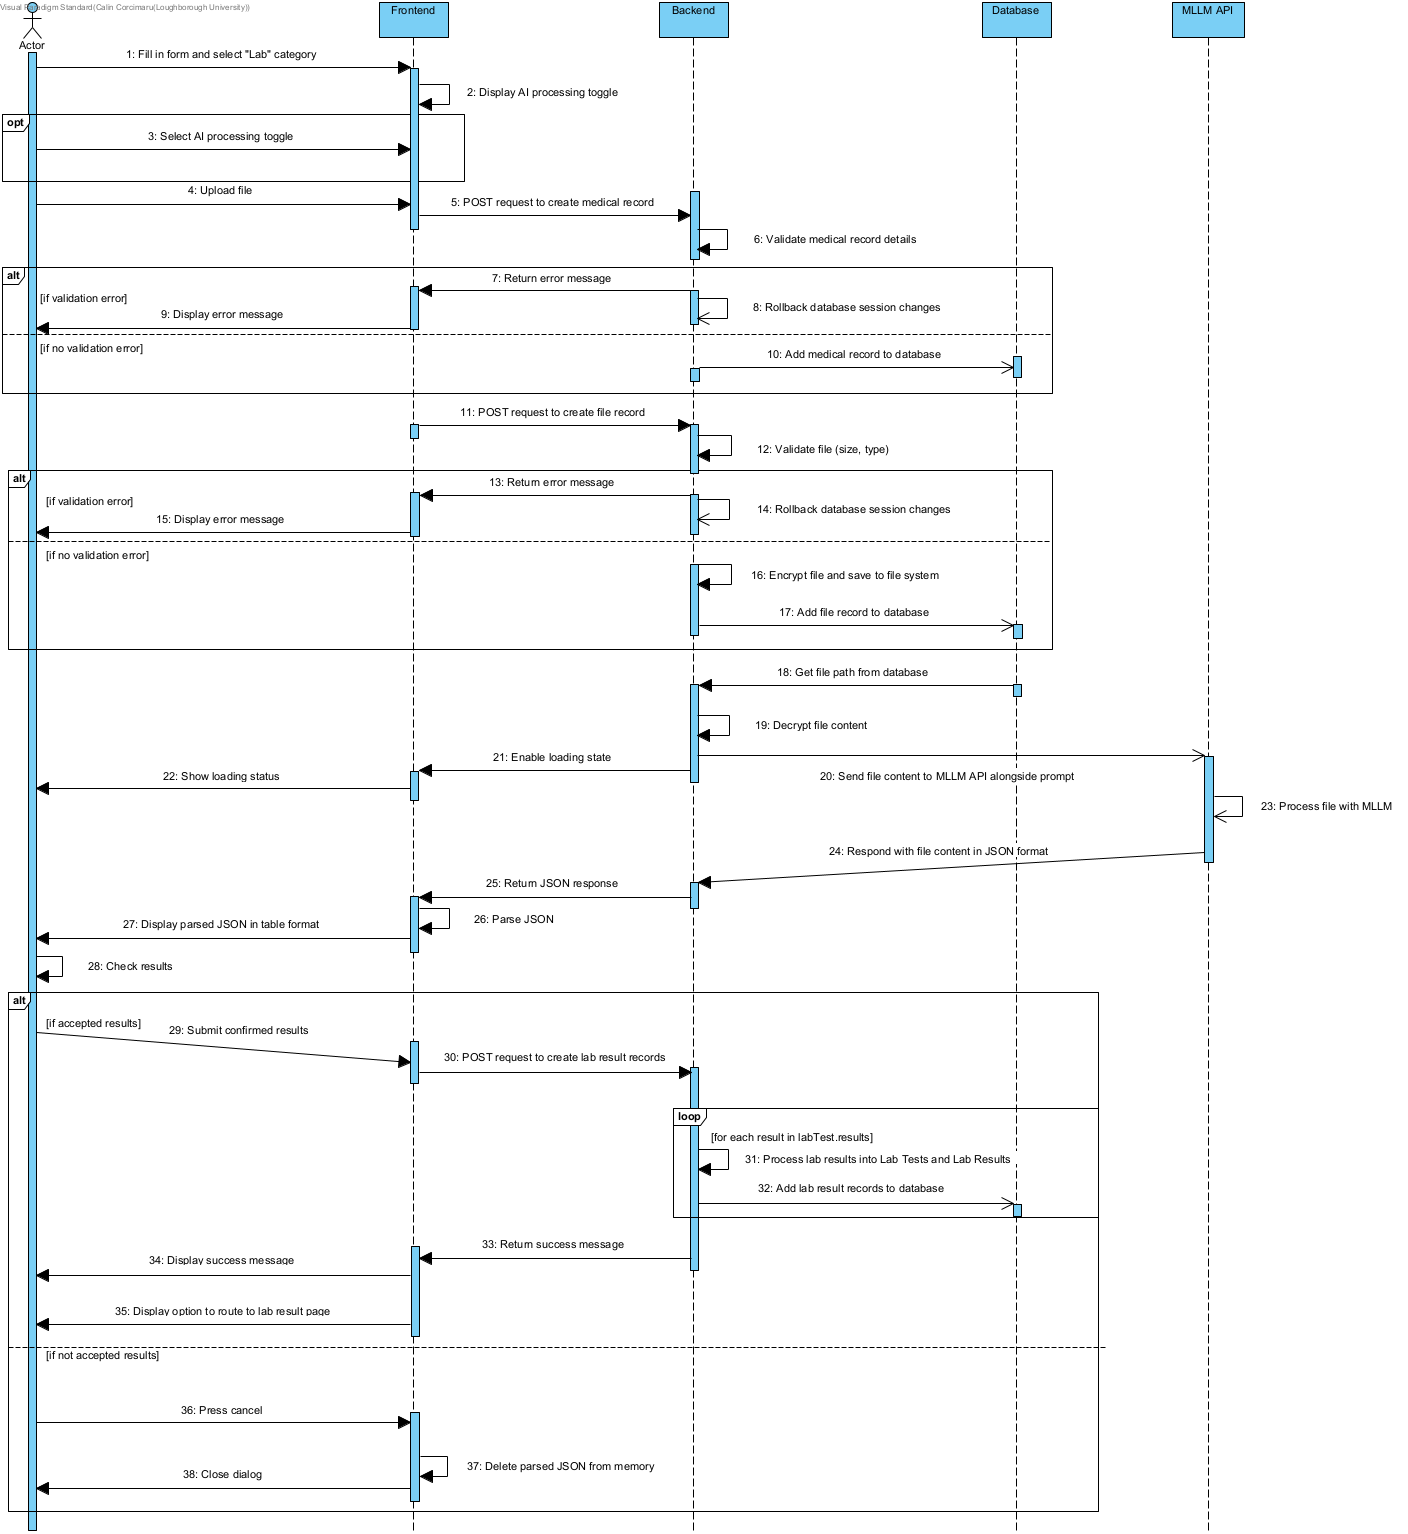
\includegraphics[width=\textwidth,height=0.8\textheight,keepaspectratio]{Sequence_lab.png}
  \caption{UML Sequence Diagram --- Extracting Lab Results}\label{fig:sequence_lab}
\end{figure}

\subsection{Lab Tests Extraction}

The implementation of initial lab extraction steps leveraged previously added components in sprint \#4, to streamline the user experience and maintain a single entry point for document uploads with optional AI processing. As such, the `Add Health Record' component and the `Laboratory' health record type were reused to expand the document upload flow. Upon selecting the `Laboratory' category, the user would get the option to toggle document AI processing, which will send the file to the MLLM API\@. This design choice closely matched the initial wireframe design for the `New Document' dialog, which can be seen in figure~\ref{fig:newDoc_wireframe}. As such, the updated `Add Health Record' dialog can be seen in figure~\ref{fig:labs_addDoc}.

\begin{figure}[ht]
  \centering
  \subfloat[Desktop version]{%
      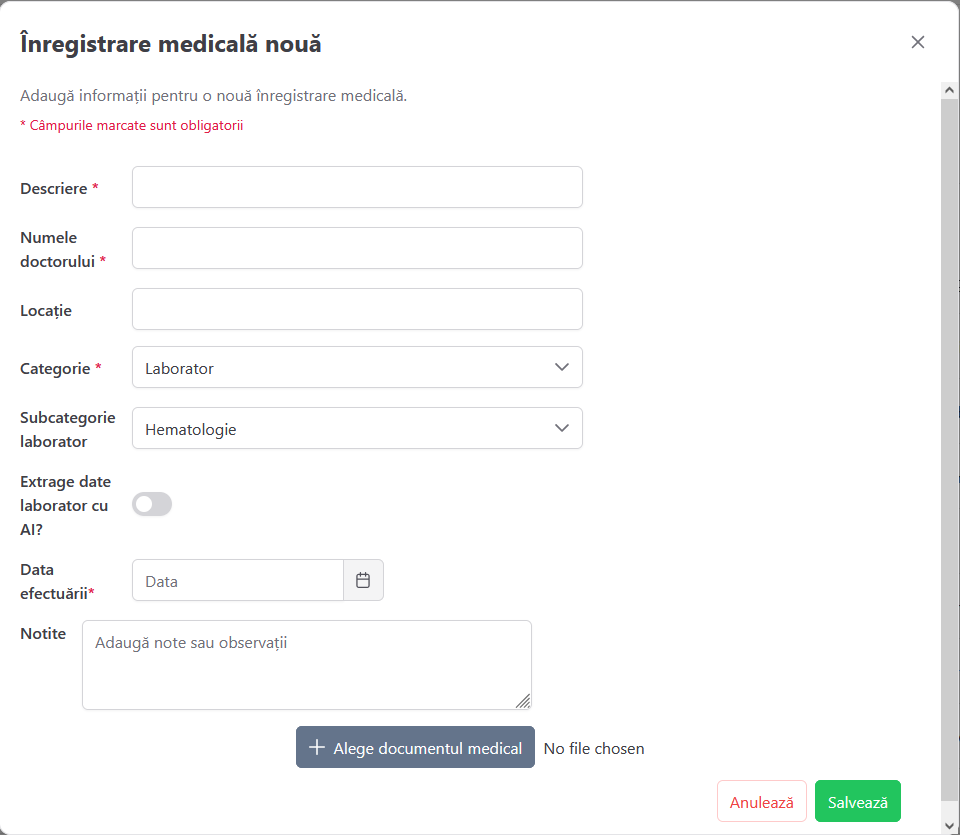
\includegraphics[width=0.7\textwidth]{Desktop_AddDoc_Labs.png}%
  }
  \\[\baselineskip]
  \subfloat[Mobile version]{%
      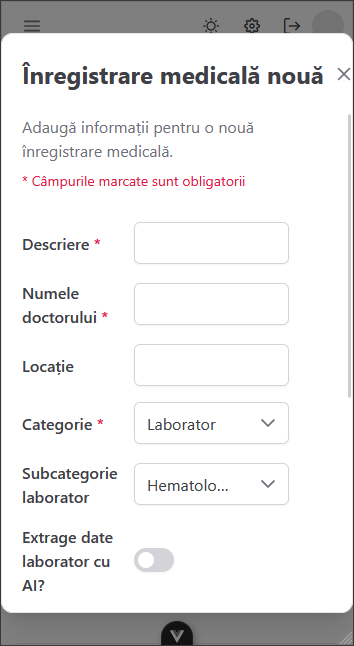
\includegraphics[width=0.3\textwidth]{Mobile_AddDoc_Labs.png}%
  }
  \caption{Desktop and Mobile version of the new Add Document dialog}\label{fig:labs_addDoc}
\end{figure}

\FloatBarrier{}

Google's Gemini 2.0 Flash was selected as the application's MLLM, based on research of available free tiers with API access from table~\ref{tab:llm_apis}. However, it was noted that a local MLLM could've also been used for the project, a point which will be discussed in more detail in section~\ref{sec:future_work}. The MLLM implementation mainly involved using Prompt Engineering techniques to provide explicit instructions and format the output consistently. Prompting techniques from section~\ref{sec:prompt} were used to write the following prompt, which is passed alongside the file to the API:

\begin{lstlisting}[language=Python, caption=Prompt for Lab Results Extraction]
def extract_with_llm(file_content: bytes, file_type: str):
  prompt = """You have been given a document that contains lab results that is written in the Romanian language. Your job is to extract all lab results from this document in JSON format with the following fields: test_name, test_code, value, unit, reference_range, method. Sometimes the code of the test will be in the name itself, and it is your job to determine if the code is there, for example in brackets or separated by a comma, and separate the name and the code. Sometimes the lab result will not have a method specified, and in that case you return an empty string. The document is in Romanian, however the JSON keys should be in English.

  EXTREMELY IMPORTANT FORMATTING INSTRUCTIONS:
  1. Return ONLY the raw JSON array
  2. DO NOT use code blocks, backticks, or markdown formatting
  3. DO NOT include ```json or ``` anywhere in your response
  4. DO NOT include any explanations or text before or after the JSON
  5. Your response must start with the '[' character and end with the ']' character
  6. The output should be valid JSON that can be parsed directly
  7. Use period (.) as the decimal separator, not comma (,)

  Example of how your output should look, starting from the very first character:
  [{"test_name":"Hemoglobina","test_code":"HGB","value":"14.3","unit":"mg/dL","reference_range":"13.2-17.3", "method":"Chemiluminiscenta"}]
  if there is no method specified, return an empty string:
  [{"test_name":"Hemoglobina","test_code":"HGB","value":"14.3","unit":"mg/dL","reference_range":"13.2-17.3", "method":" "}]"""  
\end{lstlisting}

Upon receiving the results in a JSON format, the system would parse the response and display it in a table format to the user. Next, a validation step was added to ensure result accuracy before submitting the data to the backend, by utilising PrimeVue's DataTable row editing feature to enable the user to correct the results if necessary. This step was deemed necessary to ensure any possible MLLM hallucination could be corrected by the user. An example of how the extracted lab results are displayed can be seen in figure~\ref{fig:labs_extracted}.

\begin{figure}[htbp]
  \centering
  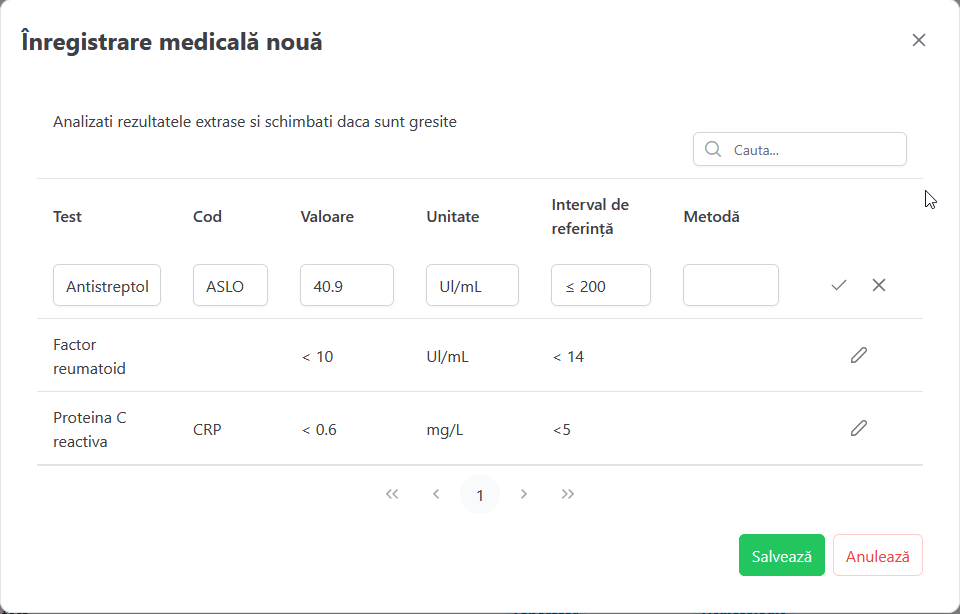
\includegraphics[width=\textwidth]{Desktop_Validate_Labs.png}
  \caption{Desktop dialog validation of extracted lab results}\label{fig:labs_extracted}
\end{figure}

The extracted lab results also leverage DataTable's dynamic column generation feature, ensuring the ability to accommodate any set of columns passed by the result data. This is important, as it may not be possible to predict the number of columns beforehand, but it also greatly simplifies the code needed to create the table. A code snippet of the DataTable can be seen below:

\begin{lstlisting}[language=HTML, caption=Dynamic DataTable for Lab Results]
  <DataTable
    :value="extractionResult"
    v-model:editingRows="editingRows"
    class="w-full"
    :rows="10"
    editMode="row"
    paginator
    dataKey="test_name"
    @row-edit-save="onRowEditSave"
    v-model:filters="filters"
    :globalFilterFields="['test_name', 'test_code']">
    <template #header>
      <h2 class="m-0">Analizati rezultatele extrase si schimbati daca sunt gresite</h2>
      <div class="flex justify-end">
        <IconField>
          <InputIcon>
            <i class="pi pi-search" />
          </InputIcon>
          <InputText
            size="small"
            v-model="filters['global'].value"
            placeholder="Cauta..."/>
        </IconField>
      </div>
    </template>
    <Column 
      v-for="col of columns" 
      :key="col.field" 
      :field="col.field" 
      :header="col.header">
      <template #editor="{ data, field }">
        <InputText v-model="data[field]" class="w-full" fluid />
      </template>
    </Column>
    <Column
      :rowEditor="true"
      style="width: 10%; min-width: 8rem"
      bodyStyle="text-align:center"/>
  </DataTable>
\end{lstlisting}

\subsubsection{Backend changes}

To accommodate the new lab extraction feature, the database was extended with two new tables: LabTest, which contained the core test metadata (name and code) and LabResult, which contained individual test results with values, units and reference ranges. A dual table approach was chosen to prevent data duplication and facilitate historical tracking by allowing to associate multiple results to one test type. The updated database can be seen in figure~\ref{fig:erd_s5}. It includes a direct patient-result relationship to optimise queries for cases when retrieving all lab results for a patient is necessary, as is the case for the dashboard.

A code snippet of the endpoint that handles the processing of lab results can be seen below:

\begin{lstlisting}[language=Python, caption=Lab Results Endpoint]
  # Create the lab test records in the database
@router.post('/me/labtests/')
async def create_lab_tests(extraction_result: LabsCreate, user_id: uuid.UUID = Depends(validate_session), session: Session = Depends(get_session)):
    medhistory = session.get(MedicalHistory, extraction_result.medicalhistory_id)
    user = session.get(User, user_id)
    
    if not medhistory:
        raise HTTPException(status_code=status.HTTP_404_NOT_FOUND, detail="Medical history not found")
    
    if medhistory.user_id != user_id:
        raise HTTPException(status_code=status.HTTP_403_FORBIDDEN, detail="Not authorised to access this medical history")
    
    for lab_item in extraction_result.lab_tests:
        lab_test = session.exec(select(LabTest).where(LabTest.name == lab_item.name)).first()
        
        if not lab_test:
            lab_test = LabTest(
                name = lab_item.name,
                code = lab_item.code,)
            session.add(lab_test)
            session.flush()
        
        lab_result = LabResult(
            value = lab_item.value,
            is_numeric = check_is_numeric(lab_item.value),
            unit = lab_item.unit,
            reference_range = lab_item.reference_range,
            date_collection = extraction_result.date_collection,
            test = lab_test,
            medicalhistory = medhistory,
            user = user,
            method = lab_item.method)
        
        session.add(lab_result)
        session.flush()
        
    session.commit()
    
    return {"status": status.HTTP_201_CREATED, "message": "Lab tests created successfully"}
\end{lstlisting}

\noindent\begin{minipage}{\textwidth}
  \begin{center}
      \rotatebox[origin=c]{270}{
          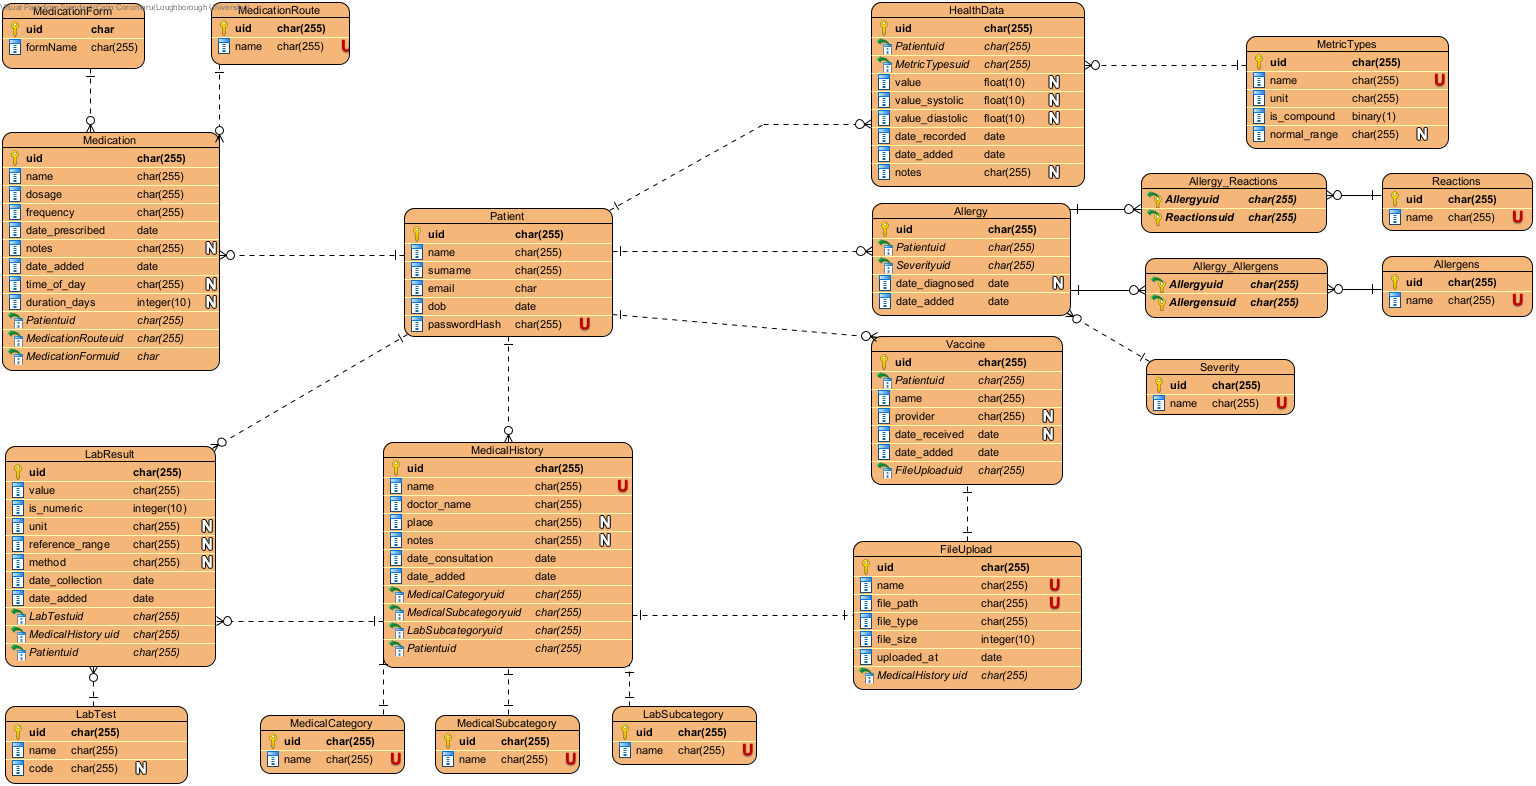
\includegraphics[width=0.95\textheight,keepaspectratio]{ERD_updatedS5.png}
      }
      \captionof{figure}{Updated Entity Relationship Diagram \- Sprint \#5}\label{fig:erd_s5}
  \end{center}
\end{minipage}

\subsection{Results visualisation}

The initial idea to display the extracted lab results was to reuse the existing design from the vitals page, developed in sprint \#3, which would've also followed the initially agreed wireframes and design. However upon discussing with stakeholders, a new design was proposed which used a hierarchical format, with expandable rows for each test type. Alongside each test type a small graph would be displayed to show the evolution of test results over time, with a visual indicator on the side which would inform patients if the recent result was outside the reference range. An example of the new lab results page can be seen in figures~\ref{fig:labs_page} and~\ref{fig:labs_page_mobile}.

This new design offered several advantages:

\begin{enumerate}
  \item A compact presentation of large amounts of test results
  \item Efficient filtering for existing test types
  \item Integrated trend visualisation through sparklines and reference range indicator
  \item A more responsive design for mobile users
\end{enumerate}

\begin{figure}[ht]
  \centering
  \subfloat[Desktop version]{%
      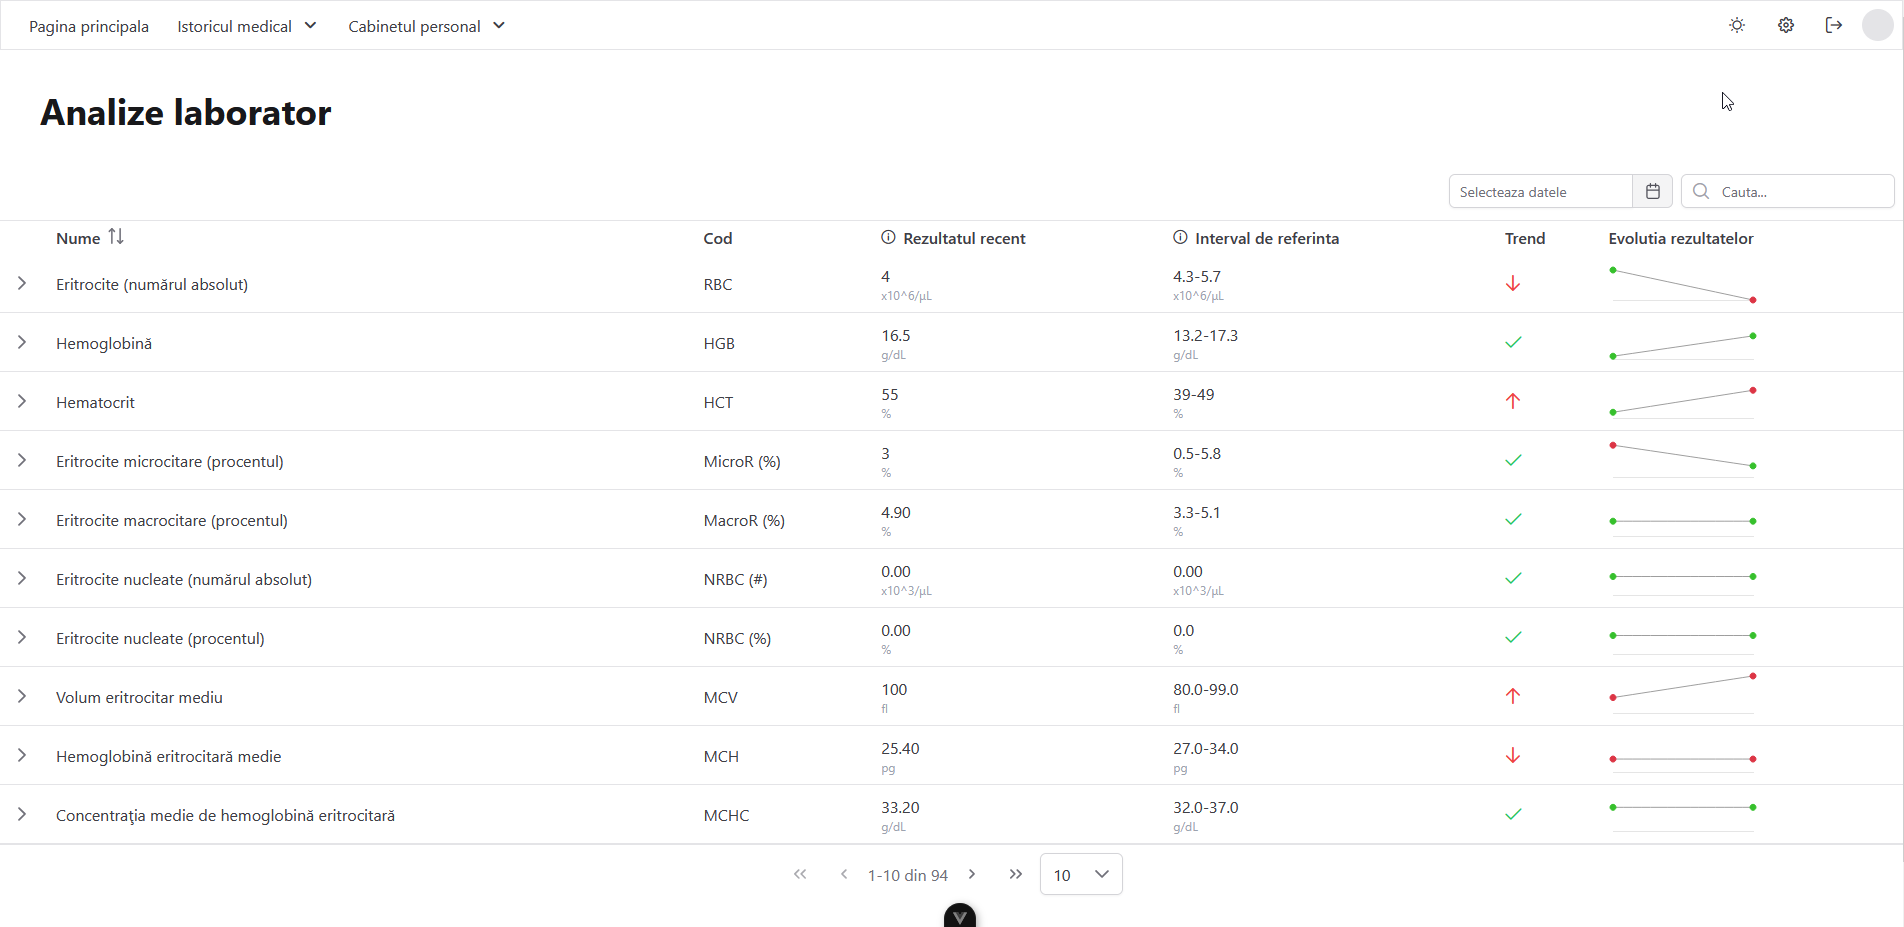
\includegraphics[width=0.9\textwidth]{Desktop_LabView.png}%
  }
  \\[\baselineskip]
  \subfloat[Desktop version \#2]{%
      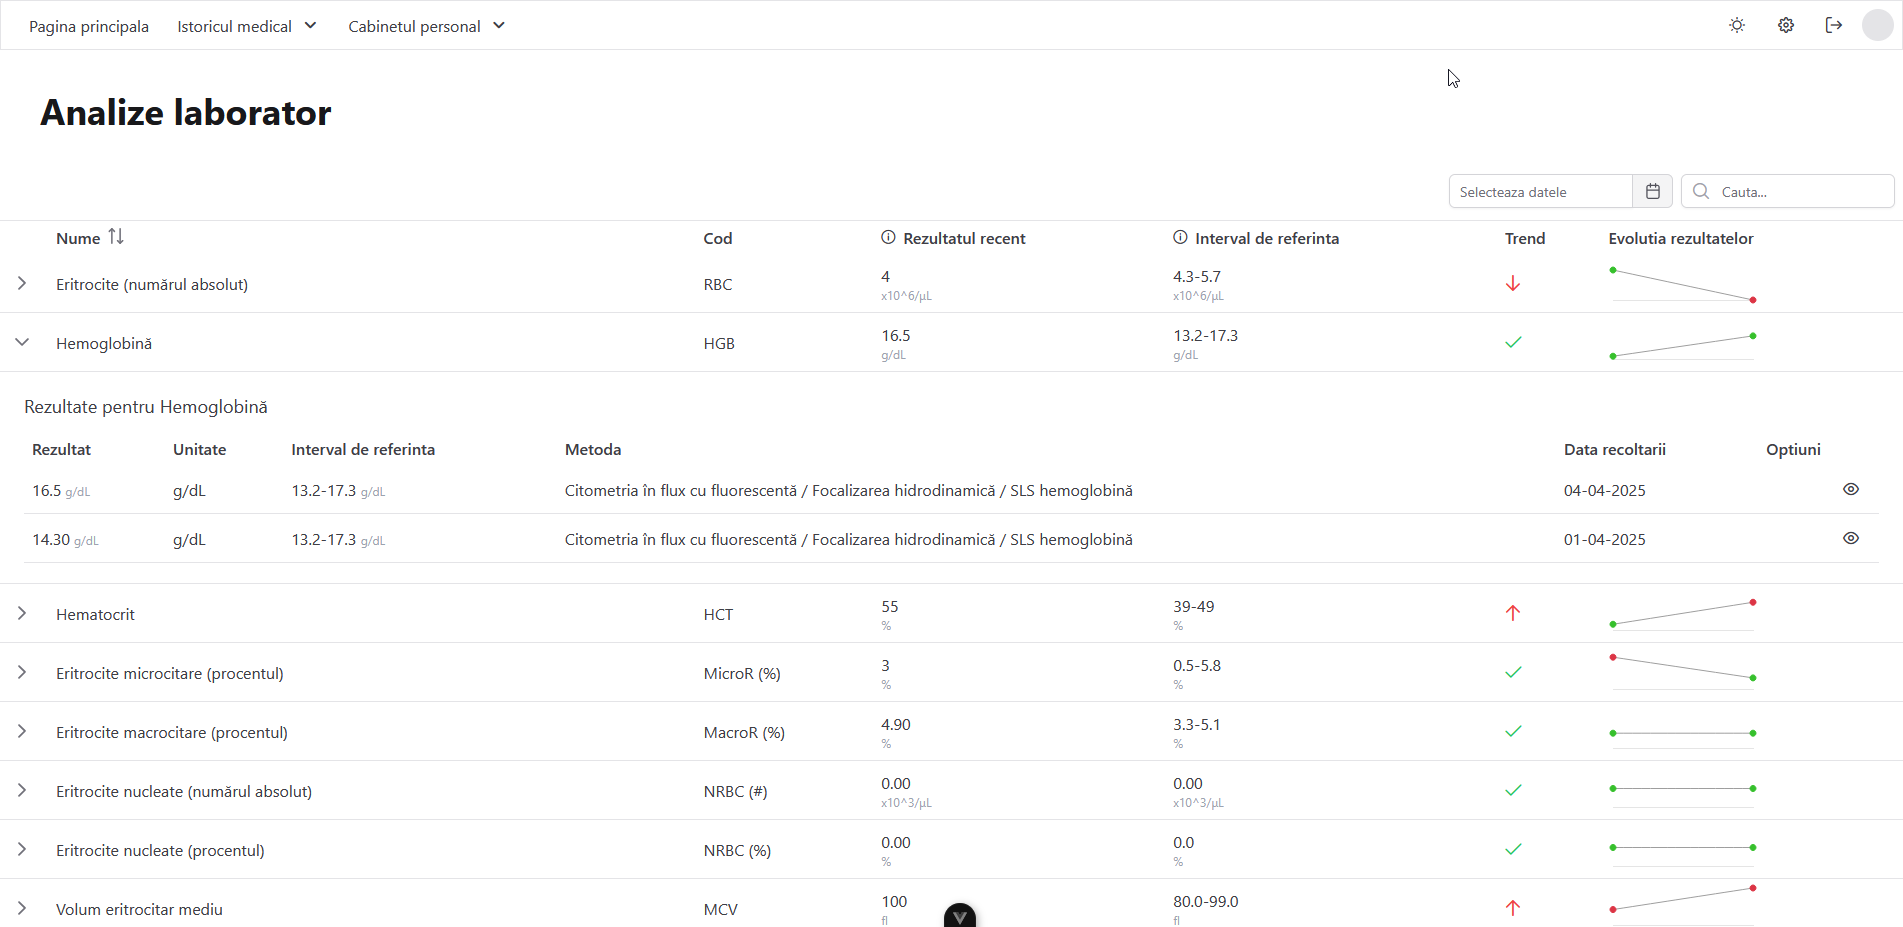
\includegraphics[width=0.9\textwidth]{Desktop_LabView2.png}%
  }
  \caption{Desktop version of the new Lab View page}\label{fig:labs_page}
\end{figure}

\begin{figure}[ht]
  \centering
  \subfloat[Mobile version]{%
      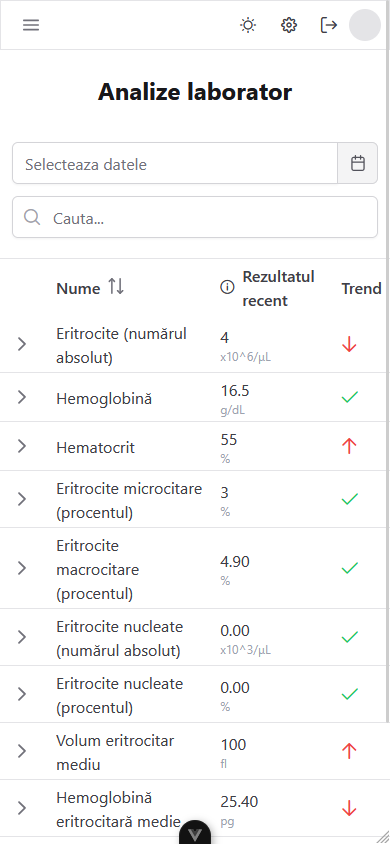
\includegraphics[width=0.4\textwidth]{Mobile_LabView.png}%
  }
  \hfill
  \subfloat[Mobile version \#2]{%
      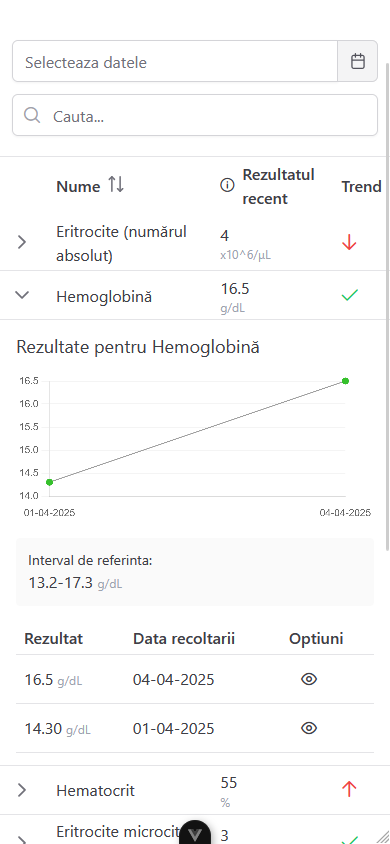
\includegraphics[width=0.4\textwidth]{Mobile_LabView2.png}%
  }
  \caption{Mobile version of the new Lab View page}\label{fig:labs_page_mobile}
\end{figure}

\subsection{Challenges encountered}

The primary challenge encountered this sprint was adapting to the mid-sprint lab result visualisation design change that was requested by the stakeholders. While it introduced additional design and research work, the agile approach taken and PrimeVue's extensive component library facilitated an effective implementation. In the end, the design actually streamlined the development as it leveraged the DataTable's capabilities for complex data presentation. Another challenge was the project's timeline constraints, which resulted in core functionality being prioritised over implementing more experimental features.

\subsection{Requirements completed}

\begin{itemize}
  \item The system must provide an overview of the patient history through 3 main sections: personal information, lab tests, and doctor consultations.
  \item The system must allow the user to view blood tests in a graphical format.
  \item The system must allow the user to view blood tests in a numerical, tabular format.
  \item For blood test results, the system should display the normal range values for each test.
  \item The system could allow the user to view the document from which the lab results were extracted.
\end{itemize}

\section{Sprint \#6}

The final sprint focused on implementing the record sharing functionality, a critical feature that would enable patients to securely share their medical records with healthcare practitioners. This feature addressed one of the core objective of this project, which was to eliminate information siloing across Moldova's multiple healthcare institutions. Instead, this feature would empower the user, creating a patient-controlled approach that complements existing institutional systems. It also represented a consolidation of previously implemented features, leveraging existing components and endpoints to display records to healthcare practitioners. 

\subsection{Share links}

During discussion with stakeholders, links were quickly identified as the preferred method of sharing medical information. Links were chosen due to their accessibility, as most doctors in Moldova have access to a computer at their desk. Similarly, links can be very versatile in how they are communicated: via email, dictated or even generated as a QR code.

To ensure a safe sharing process, the mechanism was designed with three security layers in mind. The first layer would be a random 8-character alphanumeric code, implemented to facilitate easy sharing while maintaining reasonable security. An example of a share link would be \textit{https://example.com/share/7zSaQbBd}, with the code for the link generation and token model available below:

\begin{lstlisting} [language=Python, caption=Share Link Generation]
  # Helper function to generate random strings for share codes
def generate_random_string(length: int) -> str:
    characters = string.ascii_letters + string.digits
    return ''.join(secrets.choice(characters) for _ in range(length))

# Share Token model for database
class ShareToken(SQLModel, table=True):
    id: uuid.UUID =Field(default_factory=uuid.uuid4, primary_key=True)
    share_code: str = Field(index=True, unique=True, default_factory=lambda: generate_random_string(8))
    expiration_time: datetime
    created_at: datetime = Field(default_factory=datetime.now)
    hashed_pin: str
    shared_items: dict = Field(default_factory=dict, sa_column=Column(JSON))
    user_id: uuid.UUID = Field(foreign_key="user.id")
    user: "User" = Relationship(back_populates="share_tokens")
\end{lstlisting}

The second layer was a configurable expiration period, which by default was 1 hour but could be set to a maximum of 24 hours. It was implemented to limit any potential exposure of the shared information, aligning with the single-use nature of the links during consultations. Finally, the third layer was a user-defined 6-character PIN, set during the initial steps of the share process. The PIN would be hashed and stored in the database for increased security. When accessed, the system first validates the link's expiration time, then prompts for the correct PIN before displaying any medical data. The verification endpoint is shown below:

\begin{lstlisting}[language=Python, caption=Share Link Endpoint]
  @router.post("/share/{share_code}/verify", status_code=status.HTTP_200_OK, response_model=ShareItemsResponse)
  @limiter.limit("5/minute")
  async def verify_share_token(
    request: Request, share_code: str, pin: Annotated[str, Body(embed=True)],
    session: Session = Depends(get_session)):
    share_token = session.exec(select(ShareToken).where(ShareToken.share_code == share_code)).first()
    
    if not share_token:
      raise HTTPException(status_code=status.HTTP_404_NOT_FOUND, detail="Share token not found")
    
    if not verify_hash(pin, share_token.hashed_pin):
      raise HTTPException(status_code=status.HTTP_403_FORBIDDEN, detail="Invalid PIN")
    
    user = session.exec(select(User).where(User.id == share_token.user_id)).first()
    user_data = {"name": user.name, "dob": user.dob.strftime("%d-%m-%Y") if user.dob else None}
    items_data = get_item_data(share_token.shared_items, session)
    
    return ShareItemsResponse(
      expiration_time=share_token.expiration_time,
      patient=user_data,
      items=items_data)
\end{lstlisting}

The whole record sharing flow is illustrated in sequence diagrams~\ref{fig:sequence_share_updated} and~\ref{fig:sequence_share_access}.

\begin{figure}[htbp]
  \centering
  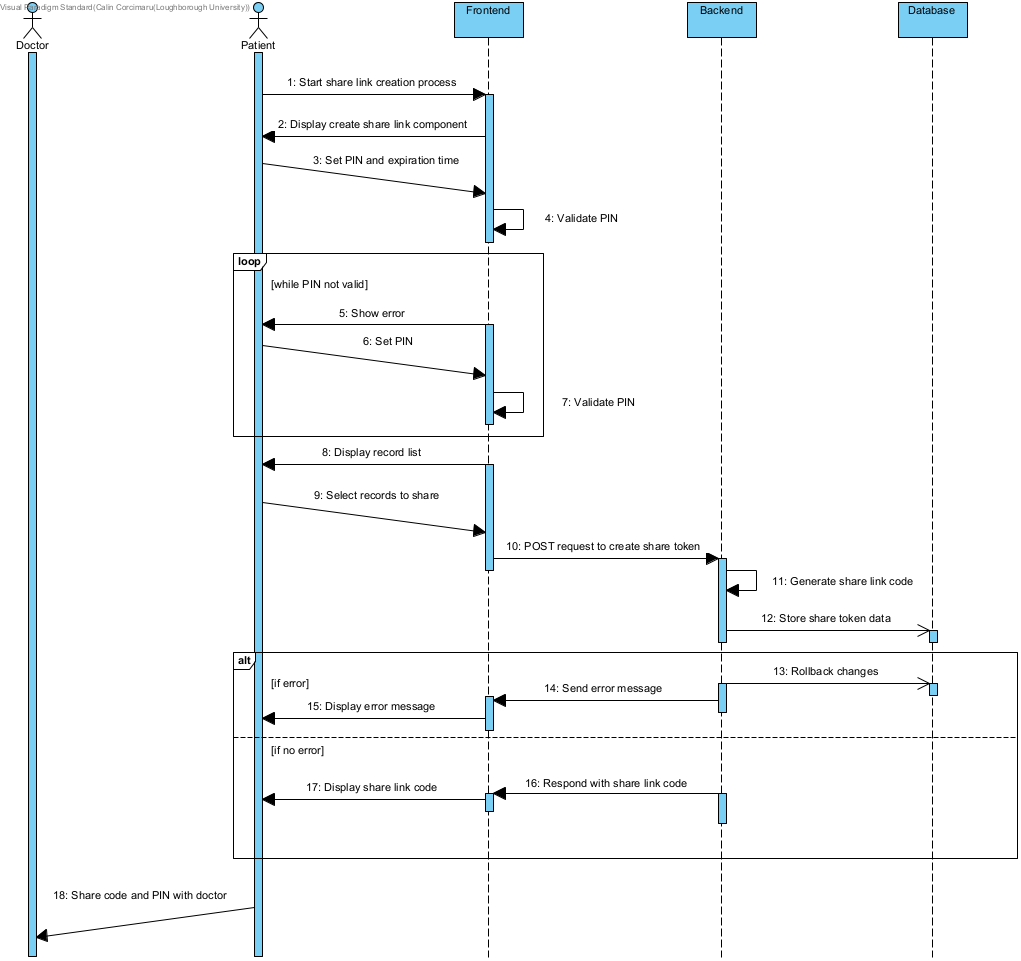
\includegraphics[width=\textwidth,height=0.8\textheight,keepaspectratio]{Sequence_share_updated.png}
  \caption{UML Sequence Diagram --- Creating share link}\label{fig:sequence_share_updated}
\end{figure}

\begin{figure}[htbp]
  \centering
  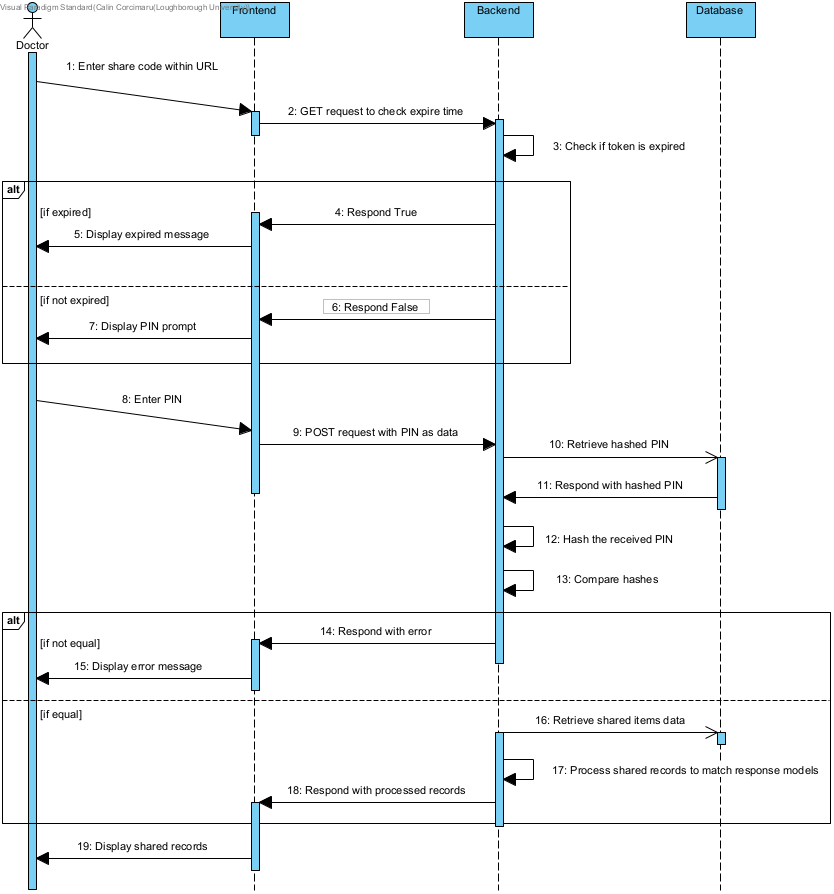
\includegraphics[width=\textwidth,height=0.8\textheight,keepaspectratio]{Sequence_share_access.png}
  \caption{UML Sequence Diagram --- Accessing shared link}\label{fig:sequence_share_access}
\end{figure}

\FloatBarrier{}

\subsection{User interface implementation}

Based on initial wireframes designs, the link creation component was located in the dashboard. To ensure a streamlined user experience, the share creation process was structured as an easy to follow and guided three-step process. The first step involved configuring the expiration time and setting the PIN, which can be seen in figure~\ref{fig:share_create}. The second step allowed users to choose the specific records to share with healthcare practitioners, displayed in figure~\ref{fig:share_records}. The final step confirmed the share link creation and displayed the generated link, as shown in figure~\ref{fig:share_result}.

\begin{figure}[htbp]
  \centering
  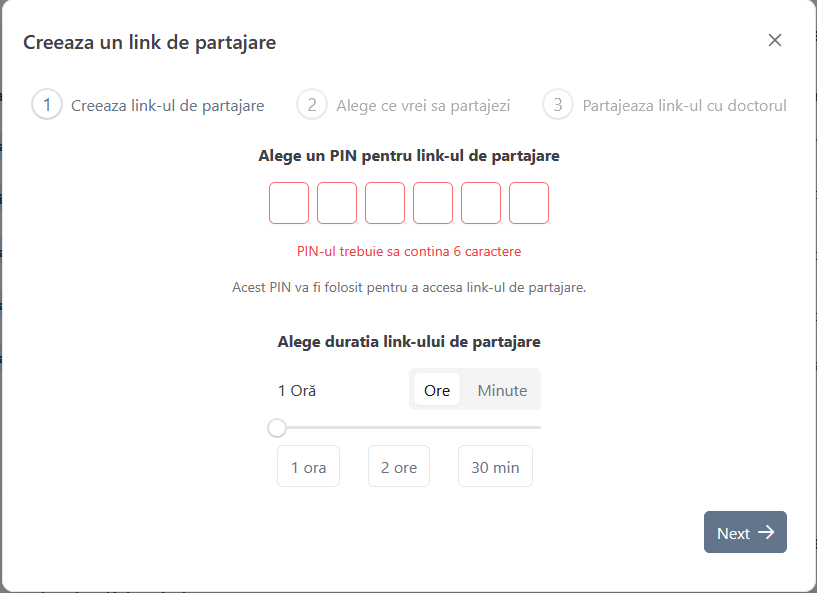
\includegraphics[width=0.9\textwidth]{Desktop_ShareCreate.png}
  \caption{1st step of share link creation}\label{fig:share_create}
\end{figure}

\begin{figure}[htbp]
  \centering
  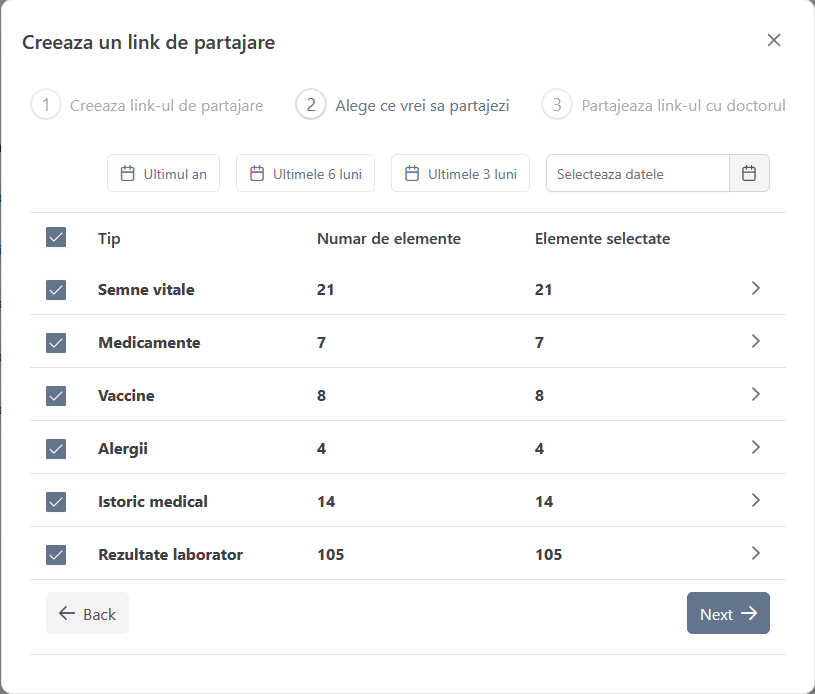
\includegraphics[width=0.7\textwidth]{Desktop_ShareRecords.png}
  \caption{2nd step of share link creation}\label{fig:share_records}
\end{figure}

\begin{figure}[htbp]
  \centering
  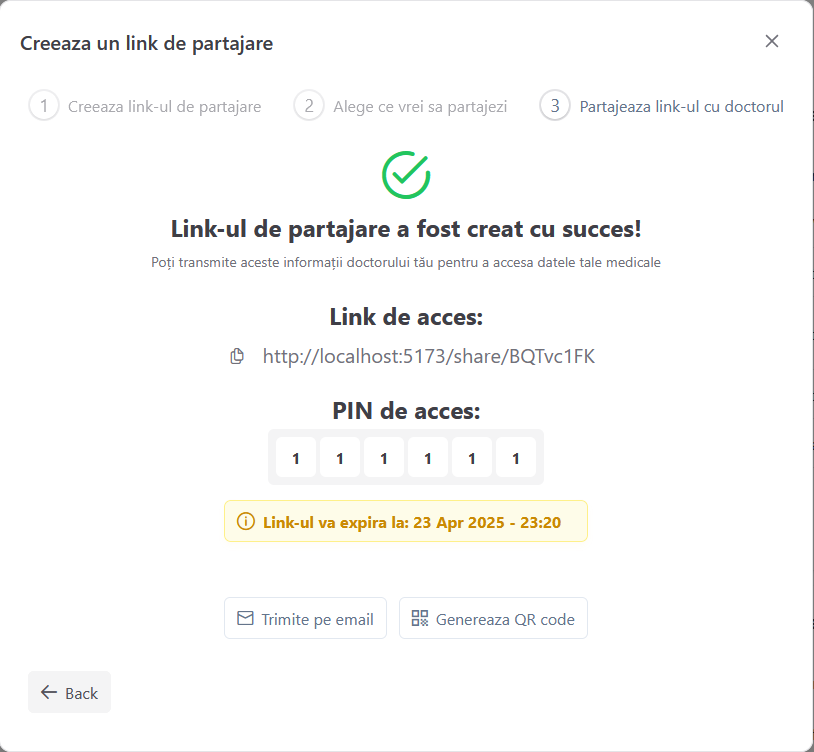
\includegraphics[width=0.7\textwidth]{Desktop_ShareResult.png}
  \caption{3rd step of share link creation}\label{fig:share_result}
\end{figure}

The frontend counterpart to the security measures was implemented next. As described in the previous section, the system would check the validity of the share link and if valid, would prompt the user to enter the PIN code. Both valid and invalid link outcomes can be seen in figures~\ref{fig:share_invalid} and~\ref{fig:share_valid}.

\begin{figure}[htbp]
  \centering
  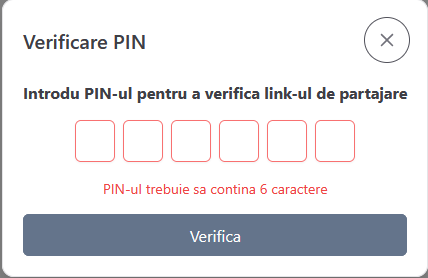
\includegraphics[width=0.7\textwidth]{Desktop_ShareValid.png}
  \caption{PIN prompt dialog}\label{fig:share_valid}
\end{figure}

\begin{figure}[htbp]
  \centering
  
\includegraphics[width=0.7\textwidth]{Desktop_ShareInvalid.png}
  \caption{Expired link dialog}\label{fig:share_invalid}
\end{figure}

The actual results page was developed last. One challenge quickly encountered was how to display the shared information in a single page. The amount of information displayed would not work with previously used methods such as PrimeVue's DataView or DataTable. Instead, TabView was used to support multiple record types onto one page.

A combination of TabView and DataTable was used to organise the different record categories --- the former would allow the user to switch different tabs representing different records (Vaccines, Allergies, etc), while the latter would contain and display the actual record data within each tab. This ensured that the user could navigate between different records without requiring a page load or additional API calls, which also greatly simplified the development process. The tabs and table columns were dynamically created based on the data received from the backend to accommodate any combination of record data.

To further expand the user experience on the shared page, basic user information and a countdown timer was added at the top of the page. An example of share page can be seen in figure~\ref{fig:share_page}.

\begin{figure}[htbp]
  \centering
  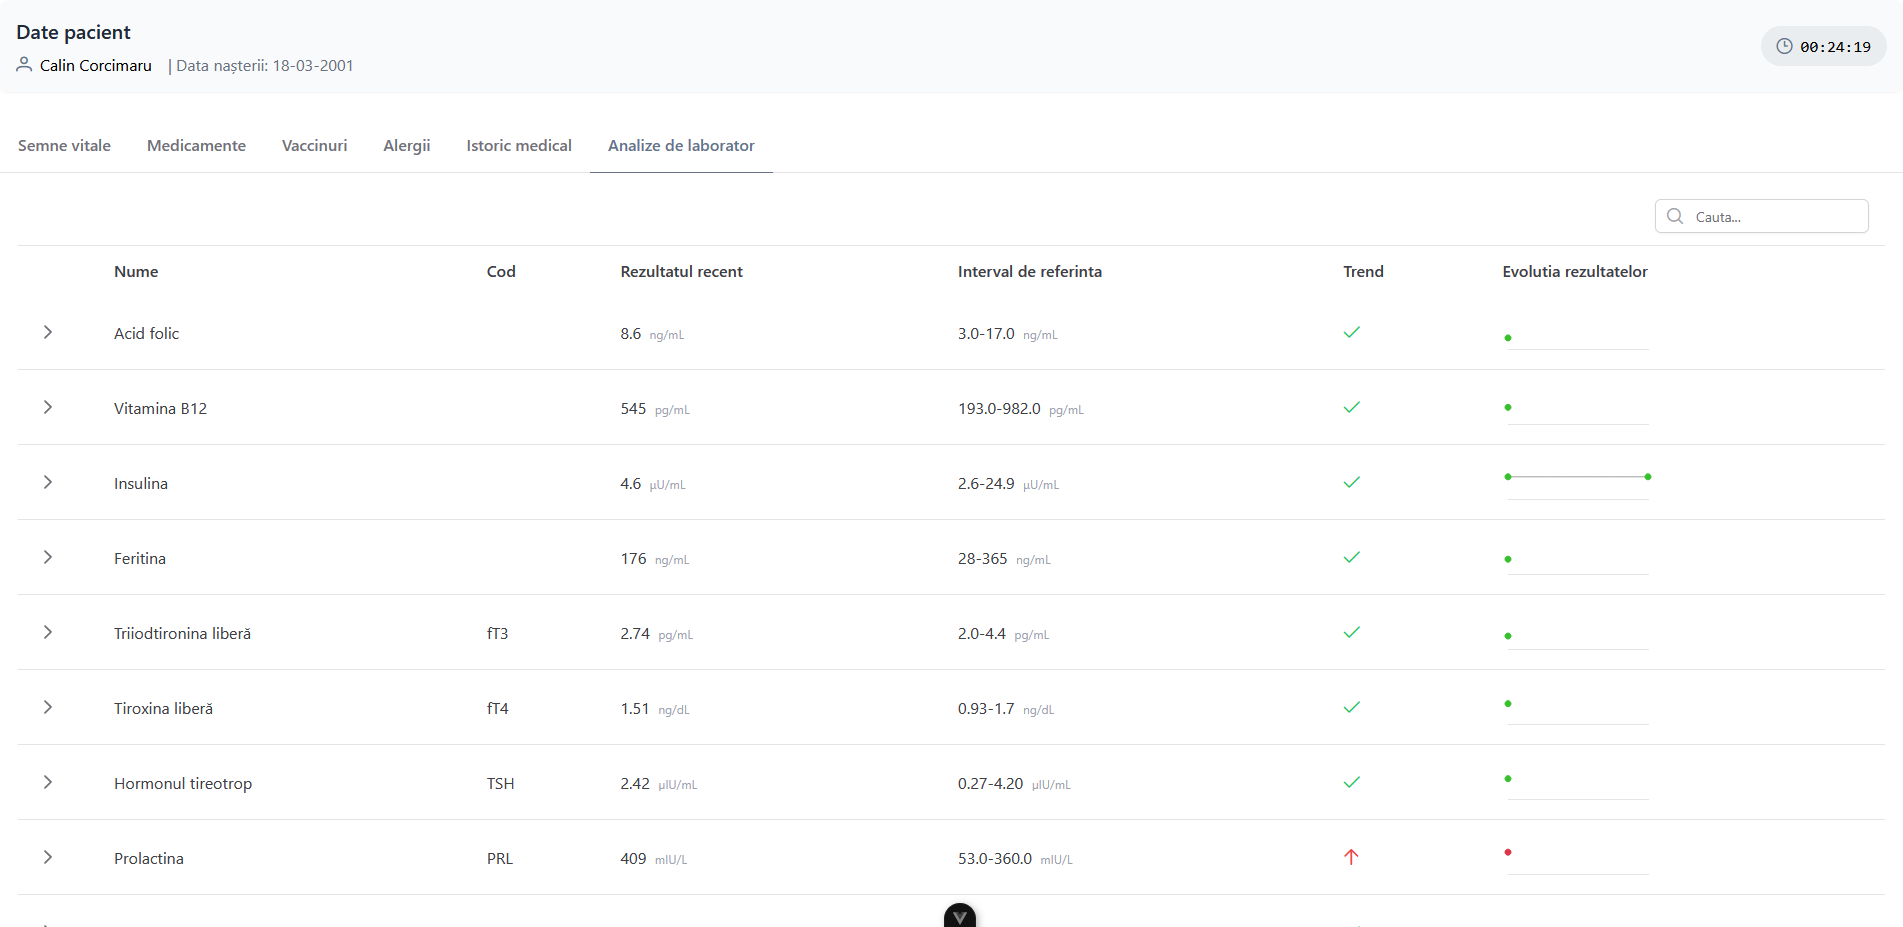
\includegraphics[width=\textwidth]{Desktop_ShareView.png}
  \caption{Share page --- Desktop version}\label{fig:share_page}
\end{figure}

\FloatBarrier{}

\subsection{Backend}

A new table was created in the database to store the share tokens, which contained metadata such as the hashed PIN, share code, expiration time and the shared items. Two different methods of storing the shared items were considered: a new table containing the record type and its respective UUID, or using a JSON field to store the shared records in the token table. The first method was quickly dismissed due to complex processing and database queries needed to be executed to retrieve and process the items into their response models. Instead, the second method was chosen, as it offered several advantages:

\begin{enumerate}
  \item Reduced processing overhead and number of database queries
  \item Storage of records in a ready-to-use format (response model)
  \item Simplified record retrieval process
  \item Future compatibility with new record types
\end{enumerate}

The updated ERD can be seen in figure~\ref{fig:erd_s6}.

\subsection{Challenges encountered}

Two notable challenges influenced this sprint's development process. Firstly, the approaching project deadline resulted in a shift in focus towards core functionality and away from additional features or refinements. This particularly affected the user interface of the share page, which was simplified to accommodate the time constraints. 

Multilingual conflicts was another challenge encountered. The combination of a Romanian frontend with an English-based database and codebase created name inconsistencies, which were especially noticeable in dynamically generated content such as table headers. This discrepancy stemmed from developing the application within a English-based academic context, while targeting a Romanian-speaking audience. While acceptable for a prototype implementation, a production system would require comprehensive internationalisation support to ensure a consistent user experience.

\subsection{Requirements completed}

\begin{itemize}
  \item The system must allow the patient to generate a shareable link to provide access to their medical records.
  \item When creating the shareable link, the system must allow the patient to set an expiration date for the link.
  \item When creating the shareable link, the system should allow the patient to set an access password for the link.
  \item When creating the shareable link, the system should allow the patient to select which records to share with the doctor.
\end{itemize}

\noindent\begin{minipage}{\textwidth}
  \begin{center}
      \rotatebox[origin=c]{270}{
          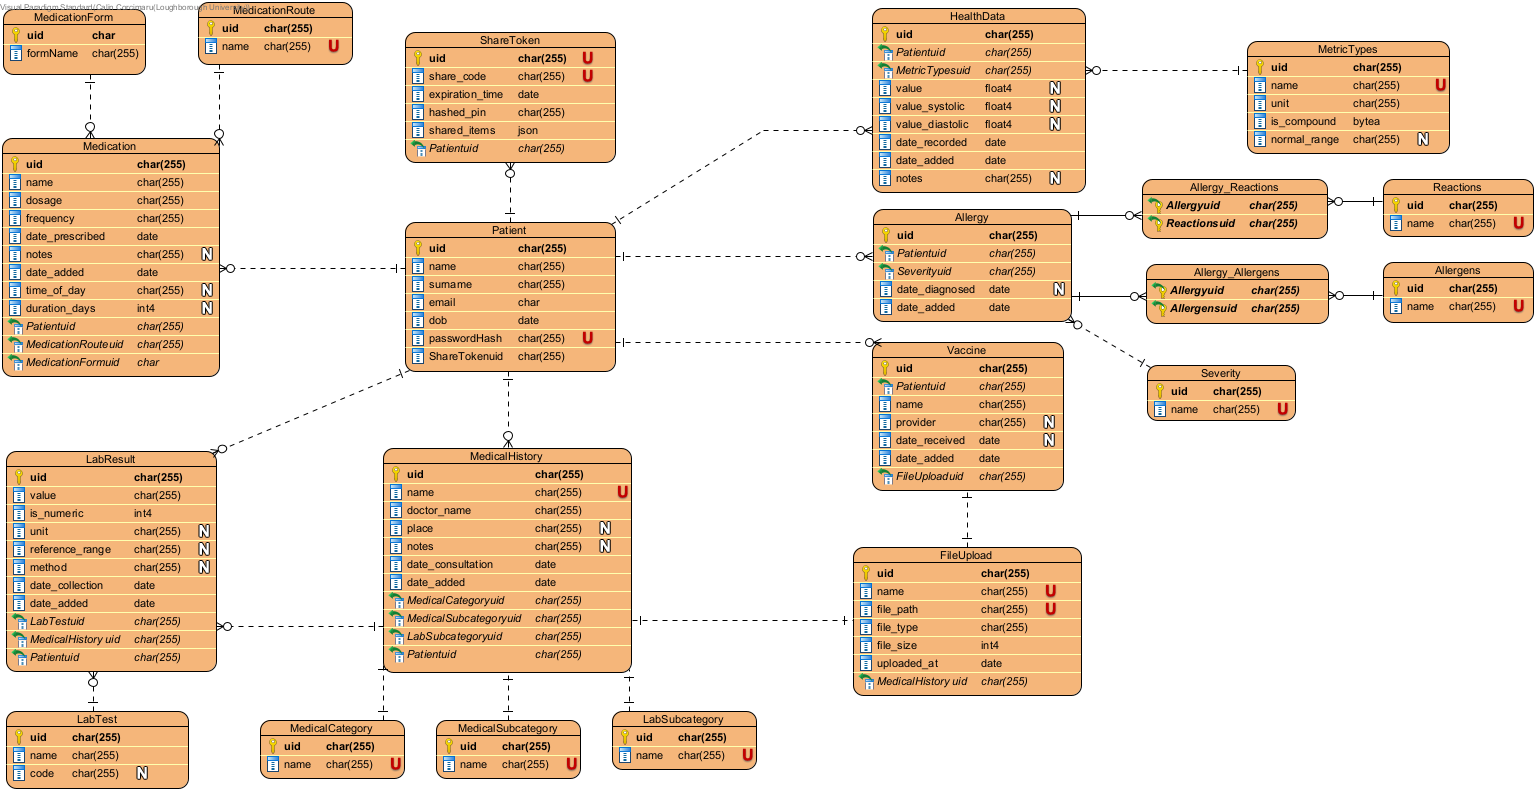
\includegraphics[width=0.95\textheight,keepaspectratio]{ERD_updatedS6.png}
      }
      \captionof{figure}{Updated Entity Relationship Diagram \- Sprint \#6}\label{fig:erd_s6}
  \end{center}
\end{minipage}